%%% Hlavní soubor. Zde se definují základní parametry a odkazuje se na ostatní části. %%%

%% Verze pro jednostranný tisk:
% Okraje: levý 40mm, pravý 25mm, horní a dolní 25mm
% (ale pozor, LaTeX si sám přidává 1in)
\documentclass[12pt,a4paper]{report}
\setlength\textwidth{145mm}
\setlength\textheight{247mm}
\setlength\oddsidemargin{15mm}
\setlength\evensidemargin{15mm}
\setlength\topmargin{0mm}
\setlength\headsep{0mm}
\setlength\headheight{0mm}
% \openright zařídí, aby následující text začínal na pravé straně knihy
\let\openright=\clearpage

%% Pokud tiskneme oboustranně:
% \documentclass[12pt,a4paper,twoside,openright]{report}
% \setlength\textwidth{145mm}
% \setlength\textheight{247mm}
% \setlength\oddsidemargin{15mm}
% \setlength\evensidemargin{0mm}
% \setlength\topmargin{0mm}
% \setlength\headsep{0mm}
% \setlength\headheight{0mm}
% \let\openright=\cleardoublepage

%% Použité kódování znaků: obvykle latin2, cp1250 nebo utf8:
\usepackage[utf8]{inputenc}

%% Ostatní balíčky
\usepackage{hhline}
\usepackage{inconsolata}
\usepackage{paralist}
\usepackage{array}
\usepackage[shellescape]{gmp}
\usepackage{graphicx}
\usepackage{amsthm}
\usepackage{enumitem}
\usepackage[table]{xcolor}
\usepackage{tikz}
\usepackage{lmodern}
\usepackage{url}
\usepackage[T1]{fontenc}
\usepackage{listings}
\usepackage{caption}
\usepackage{colortbl}
\usepackage{amsmath}
\usepackage{pgfplots}
\usepackage{pgfplotstable}
\usepackage{dirtree}
\usepackage{ifpdf}
\usepackage{multirow}
\ifpdf
  \DeclareGraphicsRule{*}{mps}{*}{}
\fi

\bibliographystyle{plain}

\lstset {
	frame=bt,
    language=C++,
%   backgroundcolor=\color{black!5},
	backgroundcolor=\color{white},
%   numbers=left,
%   numbersep=5pt,
%	numberstyle=\tiny,
	xleftmargin=10pt,
	xrightmargin=10pt,
    basicstyle=\footnotesize\ttfamily,
    keywordstyle=\bfseries,
    aboveskip=15pt,
    belowskip=15pt,
    showstringspaces=false
}

%% Balíček hyperref, kterým jdou vyrábět klikací odkazy v PDF,
%% ale hlavně ho používáme k uložení metadat do PDF (včetně obsahu).
%% POZOR, nezapomeňte vyplnit jméno práce a autora.
\usepackage[unicode]{hyperref}   % Musí být za všemi ostatními balíčky
\hypersetup{pdftitle=Bobox Runtime Optimization}
\hypersetup{pdfauthor=Lukáš Krížik}
\hypersetup{pdfborder={0 0 0}}

\usepackage{epstopdf}

\usetikzlibrary{arrows,fit,positioning,calc,patterns,shapes.multipart,backgrounds} 
\tikzset{
    %Define standard arrow tip
    >=stealth',
    %Define style for boxes
    title/.style={
           text centered},
    % Define arrow style
    pil/.style={
           ->,
           thick,
           shorten <=3pt,
           shorten >=3pt,}
}

%%% Drobné úpravy stylu

% makro for code text definition
\def\code#1{\texttt{#1}}

% Tato makra přesvědčují mírně ošklivým trikem LaTeX, aby hlavičky kapitol
% sázel příčetněji a nevynechával nad nimi spoustu místa. Směle ignorujte.
\makeatletter
\def\@makechapterhead#1{
  {\parindent \z@ \raggedright \normalfont
   \Huge\bfseries \thechapter. #1
   \par\nobreak
   \vskip 20\p@
}}
\def\@makeschapterhead#1{
  {\parindent \z@ \raggedright \normalfont
   \Huge\bfseries #1
   \par\nobreak
   \vskip 20\p@
}}
\makeatother

% Toto makro definuje kapitolu, která není očíslovaná, ale je uvedena v obsahu.
\def\chapwithtoc#1{
\chapter*{#1}
\addcontentsline{toc}{chapter}{#1}
}

\begin{document}

% Trochu volnější nastavení dělení slov, než je default.
\lefthyphenmin=2
\righthyphenmin=2

%%% Titulní strana práce

\pagestyle{empty}
\begin{center}

\large

Charles University in Prague

\medskip

Faculty of Mathematics and Physics

\vfill

{\bf\Large MASTER THESIS}

\vfill

\centerline{\mbox{\includegraphics[width=60mm]{../img/logo.eps}}}

\vfill
\vspace{5mm}

{\LARGE Lukáš Krížik}

\vspace{15mm}

% Název práce přesně podle zadání
{\LARGE\bfseries Bobox Runtime Optimization}

\vfill

% Název katedry nebo ústavu, kde byla práce oficiálně zadána
% (dle Organizační struktury MFF UK)
The Department of Software Engineering

\vfill

\begin{tabular}{rl}

Supervisor of the master thesis: & RNDr. Filip Zavoral, Ph.D. \\
\noalign{\vspace{2mm}}
Study programme: & Informatics \\
\noalign{\vspace{2mm}}
Specialization: & Software Systems \\
\end{tabular}

\vfill

% Zde doplňte rok
Prague 2014

\end{center}

\newpage

%%% Následuje vevázaný list -- kopie podepsaného "Zadání diplomové práce".
%%% Toto zadání NENÍ součástí elektronické verze práce, nescanovat.

%%% Na tomto místě mohou být napsána případná poděkování (vedoucímu práce,
%%% konzultantovi, tomu, kdo zapůjčil software, literaturu apod.)

\openright

\noindent
I would like to thank my family and friends for a persistent support in studies. I would also like to thank the supervisor for the patience and helpful advice.

\newpage

%%% Strana s čestným prohlášením k diplomové práci

\vglue 0pt plus 1fill

\noindent
I declare that I carried out this master thesis independently, and only with the cited
sources, literature and other professional sources.

\medskip\noindent
I understand that my work relates to the rights and obligations under the Act No.
121/2000 Coll., the Copyright Act, as amended, in particular the fact that the Charles
University in Prague has the right to conclude a license agreement on the use of this
work as a school work pursuant to Section 60 paragraph 1 of the Copyright Act.

\vspace{10mm}

\hbox{\hbox to 0.5\hsize{%
In ........ date ............
\hss}\hbox to 0.5\hsize{%
signature of the author
\hss}}

\vspace{20mm}
\newpage

%%% Povinná informační strana diplomové práce

\vbox to 0.5\vsize{
\setlength\parindent{0mm}
\setlength\parskip{5mm}

Název práce:
Bobox Runtime Optimization
% přesně dle zadání

Autor:
Lukáš Krížik

Katedra:  % Případně Ústav:
Katedra softwarového inženýrství
% dle Organizační struktury MFF UK

Vedoucí diplomové práce:
RNDr. Filip Zavoral, Ph.D.
% dle Organizační struktury MFF UK, případně plný název pracoviště mimo MFF UK

Abstrakt:
Cílem této diplomové práce je vytvořit nástroj na optimalizaci kódu pro paralelní prostředí Bobox. Nástroj redukuje počet krátce a dlouze běžících úloh na základě statické analýzy kódu. Některé případy krátce běžících úloh způsobují zbytečné přeplánování. Pokud plánovač nemá dostatek informací o dané úloze, plánovač může úlohu naplánovat, i když tato úloha nemá všechna potřebná vstupní data. Pro odstranění krátce běžící úlohy nástroj analyzuje použití vstupních dat a informuje plánovač. Dlouze běžící úlohy můžou v některých případech potlačit paralelismus. Větší granularita úloh může znatelně vylepšit časy běhu v paralelním prostředí. Pro odstranění dlouze běžících úloh nástroj musí být schopen vyhodnotit složitost kódu a vložit příkaz pro přeplánování na vhodné místo.
% abstrakt v rozsahu 80-200 slov; nejedná se však o opis zadání diplomové práce

Klíčová slova:
bobox, statická analýza kódu, optimalizace, složitost kódu, clang
% 3 až 5 klíčových slov

\vss}\nobreak\vbox to 0.49\vsize{
\setlength\parindent{0mm}
\setlength\parskip{5mm}

Title:
Bobox Runtime Optimization
% přesný překlad názvu práce v angličtině

Author:
Lukáš Krížik

Department:
The Department of Software Engineering
% dle Organizační struktury MFF UK v angličtině

Supervisor:
RNDr. Filip Zavoral, Ph.D.
% dle Organizační struktury MFF UK, případně plný název pracoviště
% mimo MFF UK v angličtině

Abstract:
The goal of this thesis is to create a tool for an optimization of code for the task-based parallel framework called Bobox. The optimizer tool reduces a number of short and long running tasks based on a static code analysis. Some cases of short-running tasks cause an unnecessary scheduling overhead. The Bobox scheduler can schedule a task even though the task does not have all input data. Unless, the scheduler has enough information not to schedule such task. In order to remove such short-running task, the tool analyses its input usage and informs the scheduler. Long-running tasks inhibit a parallel execution in some cases. A bigger task granularity can significantly improve execution times in a parallel environment. In order to remove a long-running task, the tool has to be able to evaluate a runtime code complexity and yield a task execution in the appropriate place.
% abstrakt v rozsahu 80-200 slov v angličtině; nejedná se však o překlad
% zadání diplomové práce

Keywords:
bobox, static code analysis, optimization, code complexity, clang
% 3 až 5 klíčových slov v angličtině

\vss}

\newpage

%%% Strana s automaticky generovaným obsahem diplomové práce. U matematických
%%% prací je přípustné, aby seznam tabulek a zkratek, existují-li, byl umístěn
%%% na začátku práce, místo na jejím konci.

\openright
\pagestyle{plain}
\setcounter{page}{1}
\tableofcontents

%%% Jednotlivé kapitoly práce jsou pro přehlednost uloženy v samostatných souborech
\chapter{Introduction}
The Bobox project is a task-based framework for parallel computing. In such framework, short running tasks cause bigger CPU consumption by the framework itself, long running tasks can inhibit the parallel execution. A static code analysis can be used to detect and eliminate such execution paths in user code. Since the core and interface language of the Bobox framework is C++, static code analysis becomes accordingly difficult to lack of tools. This has been the biggest pitfall for any static analysis of C++ code. However, it has become less marginal with a growing support for tooling in the Clang compiler front-end~\cite{clang}. Clang exposes C++ code as a user-friendly \emph{Abstract Syntax Tree (AST)}~\cite{ast} structure.

\section{Goals}
Apart from this text, the main asset of this thesis is a tool for optimization of code using the Bobox framework. By analysing AST, the tool is able to diagnose and potentially transform user code to eliminate short and long execution paths. There is an implementation of two different patterns of an unoptimized usage in the context of this thesis. However, the tool is designed to be easily extensible with new optimization methods. Both implemented optimization methods are able to inject new code to hint Bobox internal facilities about the user code structure. The tool is implemented using the Clang tooling interface~\cite{clang-documentation}. Therefore, it inherits all Clang limitations such as its platform support.

\section{Structure of the thesis}
The second chapter begins with the brief description of the Bobox framework to familiarize a reader with its underlying mechanisms. A reader should understand why user code can be optimized using transformations mentioned later in chapters related to specific optimization methods.

The third chapter describes problems of a static code analysis firstly in general, then specifically for the C++ language since it is the core and interface language of the Bobox framework. The chapter also describes possible approaches for a static code analysis of C++ code, their advantages and disadvantages, the internal implementation, the user interface and limitations. The last section in this chapter addresses the related work.

Because the chosen approach to implement the optimizer tool was the Clang tooling interface, Chapter~\ref{chapter-clang} is dedicated to its detailed description. Tools implemented on top of the Clang front-end are provided with the abstract syntax tree representation of code. One section describes the design of this data structure and possibilities of its traversal. Possibilities of source-to-source transformations are described in the following section. The Clang front-end itself provides multiple interfaces for an implementation of static code analysis tools.

Next two chapters introduce implemented optimization methods. Each chapter contains sections with information related to the Bobox framework, a detailed description of algorithms used to detect an unoptimized usage of the framework and other details of the implementation.

Chapter~\ref{chapter-design} addresses a high-level look on the tool design and some details of the optimizer implementation. The following chapter contains achieved results on described scenarios. The last chapter discusses conclusions and the future work.
\chapter{Bobox}
Nowadays, an increasing performance comes with an increasing number of computational units due to reaching to physical limits of current technologies. Parallel programming becomes more and more essential in a development of performance expensive software to use all the silicon hardware provides. The thread-based approach to achieve parallelism creates a lot of complexity for a programmer to maintain and it is also not well scalable. It becomes important to abstract the underlying parallel environment to a programmer. The Bobox framework~\cite{bobox-4, bobox} addresses this issue by providing an interface for task-based parallel programming. Such approach relieves a programmer of handling thread-based programming problems such as synchronization, most technical details (e.g., cache hierarchy, CPU architecture) and communication. Apart from that, task-based programming also allows a better hardware utilization.

According to Bednárek et al.~\cite{bobox-1}, the Bobox framework is \textit{"more useful for data processing scenarios, like database query evaluation or stream processing"}. Without further details, under the hood, the framework is implemented with a fixed number of worker threads, each one with own scheduler, two task queues for every computational unit for a better utilization of CPU caches, using the task stealing mechanism. Communication between tasks uses a column-based data model, the most significant implementation detail that favors data processing problems. Each task has zero or more inputs and zero or more outputs. A single output can be connected to zero or more inputs. A task is scheduled to be executed when it has an unprocessed input.

The Bobox framework provides a C++ library as the interface to its runtime environment. A task granularity is represented by classes derived from the Bobox base class for a task called \emph{box}.

\section{Design and terminology}
\label{bobox-terminology}
The runtime environment handles implementation details of the task-based parallel environment such as scheduling and the parallel execution of tasks, data transport and the control flow. A programmer uses a declarative way to provide the environment with \emph{model} which defines the way individual tasks are interconnected. Model is used to create \emph{model instance} which is the base for a creation of \emph{user request}. User request contains only very little additional information to model instance.

After a programmer provides user request to the environment, he has no longer control over its execution. The framework provides only information whether it has finished an execution of the request. Provided user request is divided into individual tasks. When a task is ready to be executed, it is added to the task pool. A worker thread then retrieves a task from the task pool and invokes it.

The basic element of model instance is an element representing a task, called \emph{box}. In every model instance, there is a special box called \emph{initialization box}. This box is responsible for the creation of initialization input data of other boxes in model. The framework executes this task at the beginning of a request evaluation and its only goal is to send data to its only output.

Data is sent using \emph{envelope}, a column-based data structure. An empty envelope is a special type of envelope called \emph{poisoned pill}. When box receives poisoned pill on its input, there will be no more data sent to this input. All paths of model instances are required to end in another special type of box called \emph{termination box}. When this box receives poisoned pill, the execution is finished and the pipeline is deallocated.

\section{Boxes}
\label{bobox-boxes}
Boxes, as the representation of Bobox framework tasks, are executed in three steps.

\begin{enumerate}
\item The first step is \emph{prologue}, when box creates a snapshot of its inputs and stores this snapshot in member variables so user code can access it. Prologue communicates with the runtime environment and the synchronization is necessary.
\item The second step called \emph{action} is the main place for a user code execution. User code can communicate with the runtime environment using only specific member functions, e.g., it can send envelope to its output. This approach creates a transparent parallel environment to a programmer, relieving him from issues related to the parallel execution.
\item The last step is \emph{epilogue}. The step handles scheduling of the next task based on two criteria. A task is scheduled again,

\begin{enumerate}
\item if it has got an unprocessed input and it has processed some input in the action step.
\item if it requested to be scheduled again.
\end{enumerate}

There is a reason why box is not scheduled again if it has got unprocessed input and it has not processed any input during the execution. It very likely waits for another input, e.g., the join operation in a database when a task does not execute until it has data on both inputs. The possibility to explicitly request another scheduling is there for cases when single box creates a big output. A task should not be running for a long time. It can create a big output thus congest internal buffers used for communication. A task running for a long time on a single worker thread can also create the bottleneck for a parallel execution when many other tasks wait for the input from this task.

\end{enumerate}

Boxes are main objects of the interest for optimization, because they are the main place for user code. Based on a static analysis of the action step, additional code can be injected to provide Bobox internal facilities with information about the task.

\section{Usage}
\label{bobox-usage}
To implement a Bobox task, a programmer has to inherit from the \code{basic\_box} base class. The action step is represented by one of virtual member functions from Listing~\ref{bobox-action-step}. A programmer is expected to override one of them. The synchronous version is called when all prefetched envelopes are available. The asynchronous version is called when envelope on the input which is being listened is available.

\begin{lstlisting}[caption={The code representations of the box action step.},label={bobox-action-step}]
virtual void sync_body();
virtual bool async_body(inarc_index_type inarc);
\end{lstlisting}

A programmer can also associate names to particular inputs and outputs using helper macros from the Bobox library, see Listing~\ref{bobox-macros}. Code is easier to comprehend and maintain when box inputs or outputs are referred by names instead of using indexes.

\begin{lstlisting}[caption={Helper macros for mapping of names to inputs and outputs.},label={bobox-macros}]
#define BOBOX_BOX_INPUTS_LIST(...)
#define BOBOX_BOX_OUTPUTS_LIST(...)
\end{lstlisting}

The implementation of a task is straightforward for a C++ programmer using only C++ core language features. Unfortunately, C++ syntax is not handy to express a definition of the whole execution model. The language developed to such purpose is called \emph{Bobolang}~\cite{bobolang}. Listing~\ref{bobox-bobolang} shows an example of a model definition in the Bobolang language.

\begin{lstlisting}[caption={An example of the Bobolang usage.}, label={bobox-bobolang}]
model main<()><()> {
    bobox::broadcast<()><(),()> broadcast;
    Source<()><(int)> source1(odd=true), source2(odd=false);
    Merge <(int),(int)><(int)> merge;
    Sink <(int)><()> sink;
	
    input -> broadcast;
    broadcast[0] -> source1;
    broadcast[1] -> source2;
    source1 -> [left]merge;
    source2 -> [right]merge;
    merge -> sink -> output;
}
\end{lstlisting}

\section{Cooperative scheduling}
Due to the character of the framework scheduler, user code directly affects scheduling of tasks, thus the overall performance of an execution. The framework provides ways to manipulate with task scheduling. For example, a task can give up its execution before it finishes normally. A task can also inform the scheduler that it should not be executed before all input data are available. Based on the static code analysis of user code, the optimizer tool can inject function calls into user code to affect framework scheduling.
\chapter{Static code analysis}
Detection of errors in code early in a development process is important for reducing a development cost. Most commonly used process to detect errors as soon as possible is called \emph{code review}.

Static code analysis can be considered to be an automated code review. One of the biggest pitfalls of a code review is its high price. Two or more people read code looking for a way to improve it, finding and fixing errors, performance issues, or potential errors which can become real errors in future. The quality of a code review decreases with time spent reading code. Developers need to rest to increase the quality of their code review.

Compiler warnings can be considered to be a very basic static code analysis. A compiler warns a programmer about suspicious parts of code it has detected in the compilation process. It is a good practice to turn on all compiler warnings and compile code without any detected. Most commonly used compilers provide a switch to consider warnings as errors. Software development companies often create rules to force programmers to produce warning-less code, or using the mentioned compiler switch in their development environment to implicitly remove compilation warnings.

Compilers cannot do much in diagnosing more complex errors. It is not their primary goal, which is the code compilation, and more advanced diagnostic could increase compilation times. Furthermore, there is no need to produce any binary when analysing code. Most developers of a tool for static code analysis would like to access an output of the semantic analysis. It is up to a programmer whether he reuses a compiler front-end or implements his own.

This chapter covers some of possible approaches for creating static code analysis tools. The chapter also describes the implementation of some popular analysis tools.

\section{C++ tooling}
Due to the complexity of the C++ core language, there are only very few fully C++ compliant, open-source and freeware\footnote{Proprietary compilers could do the job as well, but freeware compilers are preferred ones.} compilers. The two most known are \emph{GCC, the GNU Compiler Collection}~\cite{gcc}, and \emph{Clang/LLVM}~\cite{clang}. Apart from the standard syntax for procedural programming, C++ includes the Turing-complete template metaprogramming language. A compiler needs to \textit{execute} code in order to generate code which is eventually compiled into native code.

Based on given facts, it would be extremely difficult and unwise to individually implement own C++ front-end. The optimizer tool should use some existing front-end for the static code analysis. The set of available C++ front-ends is very limited and some of them are not suitable for a tool implementation.

\section{GCC - the GNU Compiler Collection}
GCC is a compiler with a 26 years old great history and is well established in the C++ software development world. Many helper tools for a build environment support GCC in some way, and yet programmers were struggling with writing static code analysis tools for C++. There are multiple reasons why programmers have not started using GCC. As an example, cite from \emph{Sparse FAQ}~\cite{sparse} covers their reasons for avoiding GCC: \\

\textit{"Gcc is big, complex, and the gcc maintainers are not interested in other uses of the gcc front-end.  In fact, gcc has explicitly resisted splitting up the front and back ends and having some common intermediate language because of religious license issues - you can have multiple front ends and back ends, but they all have to be part of gcc and licensed under the GPL."}\\

The first sentence, especially the first few words, is the main reason programmers have not started using the GCC front-end to create tools for a static code analysis. Some of disadvantages in using GCC for tooling are:

\begin{itemize}
\item It is very hard to learn for beginners.

\item Even though GCC consists of front-end, middle-end and back-end, it still appears to be monolithic. It is very difficult to decouple front and back ends.

\item GENERIC and GIMPLE\footnote{GENERIC and GIMPLE are names for different representations of AST. GIMPLE is a subset of GENERIC for code optimizations.} representations of code are not intuitive.

\item GCC does not keep track of tokens locations in source code, e.g., it does not keep track of macro expansions. Therefore, it is very difficult to refactor code correctly.

\item Code is optimized when it is parsed so abstract syntax tree does not correspond to source code, e.g., \code{x-x} is optimized to be \code{0}. It is extremely difficult to refactor code based on such optimized abstract syntax tree.
\end{itemize}

\section{Elsa: The Elkhound-based C/C++ Parser}
Even a smaller group of developers is able to create a relatively nice C++ compiler front-end. \emph{Elsa}~\cite{elsa} is such an example. It provides a programmer with a user-friendly AST representation of code, which is designed to be easily extensible without writing a single line of C++ code. The front-end provides a mechanism designed as the \emph{visitor pattern}. for the AST traversal. The other way to traverse a tree is to traverse a tree manually. The visitor pattern is useful for the context insensitive traversal.

The biggest disadvantage of Elsa is that its development stopped long time ago in 2005 when a different project called \emph{Oink}~\cite{oink} started. Oink uses the Elsa front-end. Later, the Oink development stopped before the year 2011 when C++ experienced its \textit{renaissance} with the new approved standard, which introduced big changes to the core language and the library. Therefore, there is almost no support for new C++11 language features. Oink as well as Elsa does not have an integrated preprocessor so it is extremely difficult to map AST with locations in source code. Elsa also suffers from a lower speed, but it would be a negligible disadvantage for smaller projects.

\section{VivaCore/OpenC++}
The \emph{VivaCore}~\cite{vivacore} library was developed as a basis for the \emph{PVS-Studio}~\cite{pvs-studio} static code analyser for C/C++. The library is derived from the older \emph{OpenC++ (OpenCxx)}~\cite{opencxx} library. The idea of using OpenC++ appeared when the team was implementing the \emph{Viva64}~\cite{vivacore} library. They were making many changes to OpenC++ and because the lack of resources, they did not continue to improve the library\footnote{Many changes did not fit into \textit{"general OpenC++ ideology"}~\cite{vivacore-ideology} so they would need to adapt and allocate new resources for such process.}. They rather developed their own library. The VivaCore library has become popular. It has been used as a basis by other popular tools such as  \emph{VisualAssist} by \emph{Whole Tomato Software}, \emph{Doxygen}, \emph{Gimpel Software PC-Lint}, \emph{Parasoft C++test} and more.

\begin{figure}[t!]
\centering
\vspace{0.5cm}
\begin{tikzpicture}[node distance=1.25cm, every text node part/.style={align=center}]
 \node(preprocessor) {External \\ preprocessor};
 \node(internal) [below=of preprocessor] {Preprocessor \\ subsystem};
 \node[below=of internal](lexer) {Lexer};
 \node[below=of lexer](parser) {Parser};
 \node[below=of parser](walker) {PT Walker};
 \node[below=of walker](metaprogram) {Metaprogram \\ subsystem};
 
 \path[<->] (preprocessor) edge node {} (internal);
 
 \path[*-*] (internal) edge node {} (lexer)
 	        (lexer) edge node {} (parser)
 	        (parser) edge node {} (walker)
 	        (walker) edge node {} (metaprogram);
 	        
 \node(utility) at (-5, -6.25) { C/C++ \\ Analysis \\ Library and \\ Utilities };
 
 \path[dashed] (utility) edge node {} (internal)
               (utility) edge node {} (lexer)
               (utility) edge node {} (parser)
               (utility) edge node {} (walker)
               (utility) edge node {} (metaprogram);
 
 \node(viva) at (-2.5, -11.5) {\LARGE\textbf{VivaCore}};
 
 \node[above=of internal, yshift=-1.25cm] (dummyfit){};
 
 \begin{pgfonlayer}{background}
  \node [draw,fit=(internal) (lexer) (parser) (walker) (metaprogram) (viva) (utility) (dummyfit)] {};
 \end{pgfonlayer}
 
\end{tikzpicture}
\caption{A design of the VivaCore library.}
\label{vivacore}
\end{figure}

Figure~\ref{vivacore} shows the library design. The library uses an external preprocessor. Without an integrated preprocessor, it is extremely hard to track macro expansions and actual locations of symbols in source code. Thus, source-to-source transformations are accordingly difficult.

A preprocessed input is passed to the library. Two library subsystems process code before it gets to the lexical analysis. The first is the input subsystem responsible for putting preprocessed code into internal data structures. The second subsystem is internally called \emph{Preprocessor}, but it does not preprocess an input in the meaning of the C++ preprocessor. It is responsible for two operations:

\begin{itemize}
\item Splitting code into strings and separating them into two logical groups. One group is for system libraries, the other group is for user code. A library user can choose whether he wants to analyse system code or just user code.
\item Removing compiler specific constructions not related to C/C++ languages, e.g., \code{SA\_Success} and \code{SA\_FormatString} are present in Visual Studio`s headers.
\end{itemize}

The next step is the lexical analysis. An output of \emph{Lexer} can be used for basic metrics or a syntax highlighting. VivaCore allows modifications to the set of tokens for the lexical analysis.

VivaCore provides a user with \emph{parse tree (PT)}, called also \emph{derivation tree (DT)}, as an output of the syntactic analysis. Parse tree differs from abstract syntax tree in the way it contains nodes representing derivation rules used in the syntactic analysis. The word \emph{abstract} comes from the reasoning that the structure hides rules used in its construction. It is actually possible to traverse PT as if it was AST. VivaCore`s PT defines two basic sets of nodes with ancestors in \code{NonLeaf} and \code{Leaf} base classes, which have \code{PTree}\footnote{\code{PTree} has \code{LightObject} as its base class used in GC.} class as their common ancestor declaring the only pure virtual member function. It is the only function necessary to be overridden in inherited classes letting their design to be more flexible.

Probably the most interesting part of the library interface is the tree traversal. There are three different \emph{walker} classes implemented for this purpose.

\begin{description}
\item[Walker] is responsible for walking over basic C++ constructions.
\item[ClassWalker] handles C++ class specific features.
\item[ClassBodyWalker] traverses a body of a C++ class.
\end{description}

It is possible to traverse PT multiple times. A user can traverse code for measurements at first. Later, in further traversals, he may modify PT. Modifying of tree nodes can trigger a tree rebuild.

The VivaCore library is one of the best libraries for the static analysis of C++ code. A relatively high number of very popular tools for the code analysis based on the library reflects its quality. Its development is still in progress and the library is still being updated. Developers also implement a support for new features introduced in new approved language standards. However, the goal of the optimizer in not only to analyse code, but also to transform user code. An external preprocessor is a major issue in using the VivaCore library.

\section{Static code analysis tools}
A code quality in big projects is hard to maintain using a code review only. If there are many code related commits every day (e.g., \emph{Crysis 2} multiplayer had $\sim$100-150 code related commits every day collecting 130 different developers over the last year of the development~\cite{crysis}), providing human resources for a code review would be inefficient. Instead of that, companies use tools for a static code analysis and diagnostic is further reviewed. However, not many companies trust tools enough to let them do source-to-source transformations, apart from formatting or simple refactoring.

This section describes some popular static code analysis tools to familiarize a reader with solutions already used to implement such tool. Even though their final goal differs from the goal of this thesis, they all have to achieve the common goal to \textit{understand} source code to some extent.

\subsection{Clang Static Analyzer}
\label{clang-analyzer}
The static analyser is a part of the Clang project implemented on top of the Clang tooling interface. The analyser is easily extensible by implementing \emph{checkers}, even though their interface may not be intuitive. Authors demonstrate how to write a simple checker for  Unix stream API in the presentation called \textit{"How To Write a Checker in 24 Hours"}~\cite{clang-analyzer-presentation}. When writing a checker, a developer needs to understand how the analyser works under the hood.

The core of the analyser does a symbolic execution of code, exploring every possible path, tracking all variables and constructing \emph{Control Flow Graph (CFG)}. Checkers participate in the CFG construction. Essentially, checkers are visitors that react on a specific set of events while traversing AST (e.g., \code{checkPreStmt}, \code{checkPostCall} functions) and eventually creating new CFG nodes.

The analyser aims to solve path-sensitive problems, e.g., problems related to the resource acquisition and release such as resource leaks and resource usage after release. The CFG construction is the core of such analysis. Actually, the development manual page of the analyser contains the important advice that discourages developers from implementing path-insensitive checkers~\cite{clang-analyzer-manual}:\\

\label{clang-analyzer-checkers}
\emph{"Some checks might not require path-sensitivity to be effective. Simple AST walk might be sufficient. If that is the case, consider implementing a Clang compiler warning. On the other hand, a check might not be acceptable as a compiler warning; for example, because of a relatively high false positive rate."}

\subsection{Clang Format}
\label{clang-format}
A consistency in code formatting is very important in big projects. It increases a readability and code becomes better machine editable. Even though consistent code formatting is very important, there are not many tools that support automatic code formatting for C++, e.g., \emph{BCPP}, \emph{Artistic Style}, \emph{Uncrustify}, \emph{GreatCode}, \emph{Style Revisor}.

The reason why companies allow the usage of automatic formatting tools is that those tools guarantee they will not change the code semantic, i.e., they edit only white space characters, literals and comments. Therefore, they will not break a compilation. There was the proposal to let clang-format reorder file includes, but it was not approved because such change can break a compilation. Main challenges for clang-format developers based on their design document were~\cite{clang-format-design}:

\begin{itemize}
\item A vast number of different coding styles has evolved over time.
\item Macros need to be handled properly.
\item It should be possible to format code that is not yet syntactically correct.
\end{itemize}

It was a hard decision for clang-format developers whether they use lexer or parser to implement such tool. Both have their advantages and disadvantages in terms of a performance, a macro management or a type information. In the end, they have decided to keep the implementation based on lexer, but there is still the ongoing discussion about adding AST information. However, this discussion is leaning towards creating a separate tool using AST, which already has the name \emph{clang-tidy}~\cite{clang-tidy}.

\subsection{OCLint}
\emph{OCLint}~\cite{oclint} is a tool implemented on top of the Clang tooling interface. It tries to create  a generic framework for code diagnostic. Main parts of OCLint are \emph{Core}, \emph{Rules} and \emph{Reporter}.

\emph{Core} controls a flow of the analysis, dispatches tasks to another modules and outputs results. It parses code, builds AST and provides modules with an access to this AST. While parsing code, it creates various metrics such as:

\begin{itemize}
\item Cyclomatic complexity.
\item NPath complexity.
\item Non-commenting source statements.
\item Statement depth.
\end{itemize}

\emph{Rules} can provide \emph{RuleConfiguration}, which defines limits for metrics. When limits are exceeded, \emph{Core} emits a violation. There are two main approaches for modules to handle diagnostic:

\begin{description}
\item[Line based] is when modules are provided with lines of code.
\item[AST based] provides modules with an access to AST using two approaches:
	\begin{itemize}
	\item Using \emph{visitor design pattern} to explore AST.
	\item Defining \emph{matchers} for suspicious code patterns.
	\end{itemize}
\end{description}

Modules are separated from \emph{Core} code thus they can be loaded in runtime. Basic diagnostic can be represented as a set of code patterns. The last task to do is to report a found diagnostic using \emph{Reporter}.

However, the pattern matching is not the strong enough mechanism to catch even a little more complex error such as a resource leak. Supported approaches other than AST matchers do not really help more than just using the Clang tooling interface directly.

\subsection{Cppcheck}
An example of a tool that does not use any compiler front-end to process source code is Cppcheck~\cite{cppcheck}. The tool does the code parsing and the analysis on its own, but the quality of understanding of source code is lower than in well-established compiler front-ends. The input for code checks is the output of the lexical analysis. Thus, it can be very difficult to implement more advanced checks. The fact that the code analysis passes only the lexical analysis phase does also mean that the tool is not able to catch even syntactic errors. Fortunately, Cppcheck implements classes such as \code{Scope} or \code{SymbolDatabase} with a functionality their names indicate.

The simplified version of a Cppcheck execution from the documentation for programmers can be written in eight steps~\cite{cppcheck-doxygen}:

\begin{enumerate}
\item Parse the command line.
\item \code{ThreadExecutor} creates necessary \code{CppCheck} instances.
\item \code{CppCheck::check} processes every file.
\item Preprocess a file inside the \code{check} member function.
    \begin{itemize}
    \item Comments are removed.
    \item Macros are expanded.
    \end{itemize}
\item Tokenize a file using \code{Tokenizer}.
\item Run all checks on the \code{Tokenizer} output called a token list.
\item Simplify a token list.\footnote{There are various simplifications applied to a token list. Every simplification passes the whole token list looking for patterns and potentially changes this list. For example, the first applied simplification changes \code{"string"[0]} to \code{'s'}. Another example is removing of \code{std::} tokens from a specific set of function calls.}
\item Run all checks on a simplified token list.
\end{enumerate}

\subsection{Summary}
Three out of four described code analysis tools are implemented on top of the Clang front-end. Cppcheck parses code by itself and cannot be considered to be a full-featured front-end. Cppcheck understands code enough to implement simple checks, but more complex analysis could become very difficult to implement.

Nonetheless, each one of the three analysis tools implemented on top of Clang has a different goal and a different \textit{view} on code from the other two tools. Such variability indicates that the Clang front-end exposes a lot of information gathered during a compilation to tools. Thus, its tooling library is a good candidate for the library used in the optimizer implementation.

\section{Related work}
There are not many tools for front-end optimizations. The main reason is that it has been a hard task to implement any front-end tool in general. Furthermore, most optimizations are already implemented in compilers. However, this thesis aims to optimize the specific framework.

\subsection{Scout}
\label{scout}
The front-end optimizer tool, called \emph{Scout}~\cite{scout}, is being developed in \emph{TU Dresden}. It is supposed to do transformations for front-end SIMD optimizations, e.g., loop auto-vectorization, a very similar task to what most current compiler back-end optimizers do. It shall transform C code into optimized C code with compiler intrinsics. Naturally, auto-vectorization is done by a compiler back-end optimizer, but there are limits to what compiler can do. It needs to use the extensive dependency and alias analysis to reason the correctness of vectorization and often rejects more complex loops. Some compilers allow programmers to annotate loops with \code{pragma} directives giving responsibility for keeping some loop invariants to programmers. A compiler can skip those checks before vectorization thus accepting more loops. Unfortunately, the measurement with the specific Intel compiler using pragma directives gave insufficient results. For example, the compiler rejected loop vectorization after the loop variable type was changed from \code{unsigned int} to \code{signed int}. Actually, Scout provides a semi-automatic vectorization, where programmers have to annotate loops using pragma directives to enable vectorization of a given loop. 

The tool provides a command line interface as well as a graphical user interface. It uses Clang to build AST from C code. AST is then transformed to different AST that represents optimized code. Finally, this optimized AST is transformed back to C code. The tool can be configured with a set of used intrinsics, i.e., \emph{SSE2}, \emph{SSE4}, \emph{AVX}, \emph{AVX2} or \emph{ARM NEON}.

\section{Summary}
All tools for a static code analysis described in this chapter were implemented by a group of programmers. Without a good library for parsing C++ code, it is an extremely difficult task to implement any tool for an analysis of C++ code. The requirement for a code transformation makes the task even harder. The lack of the C++ tooling support has been generally mentioned by programmers as one of the biggest drawbacks of using the C++ language. The situation has changed with the increased support of tooling in the Clang front-end and it is possible to implement a relatively complex tool for front-end optimizations individually or in a small group of people. The Scout tool is such example.

The Clang front-end is intentionally omitted from this chapter as the optimizer tool uses its tooling interface to analyse and transform code. The whole next chapter covers the Clang tooling interface in details. The Scout tool is the main inspiration for the decision to use the Clang front-end for an analysis and transformation since the tool has a very similar goal and its major part is implemented by a single programmer.
\chapter{Clang and tooling}
\label{chapter-clang}
A support for creating static code analysis tools for C++ was very subtle before Clang developers increased its support for tooling. All compiler front-ends were cumbersome for a usage and implementing a new front-end individually is extremely difficult. The situation has changed with Clang providing API for an access to C++ code represented as the user-friendly abstract syntax tree structure. Actually, Clang does not provide single tooling API, rather multiple APIs with differences in a usage. Differences affect mainly the way a tool accesses AST, the range of accessed information and compatibility with older versions. A tool developer can decide whether he wants to sacrifice compatibility to all information provided by front-end internals. As Clang is being developed, there is no guarantee that interfaces in their code base do not change.

The tooling interface indicates that Clang targets to diagnostic, code completion and refactoring tools. The support for source-to-source transformation is subtle. Even though there are multiple ways to transform code, most of them are deprecated.

\section{Abstract Syntax Tree}
The structure Clang provides is not only abstract syntax tree of code. It is a graph with AST nodes, but with more edges than those in AST. Clang provides mechanisms to traverse this graph as if it was AST. With an access to the AST node, a programmer is able to traverse a graph in more ways than he would be able to do with just AST structure. It allows a developer to optimize his analysing code or perform a more complex context sensitive traversal.

Unusually, the class hierarchy of nodes does not have the common ancestor. There are two large hierarchies with common ancestors in \code{Decl} and \code{Stmt} classes, some important ones with ancestors in \code{Type} and \code{DeclContext} classes, and many classes accessible only from specific nodes.

\subsection{Traversal}
\label{clang-ast-traversal}
The template responsible for the AST traversal is called \code{RecursiveASTVisitor}. It is implemented as \emph{Curiously Recurring Template Pattern (CRTP)} combined with the \emph{visitor design pattern} where a programmer is able to either react on the AST node visit or manipulate with a traversal. Due to the character of the AST nodes class hierarchy, the implementation of the visitor template is cumbersome with the extensive usage of macros. Therefore, the template has nickname \textit{macro monster}. It was promised that it will be reimplemented once so there is no guarantee that the interface will not change, even though the visitor is massively used in tools. The other approach to traverse AST is to follow edges. It is more useful in a context sensitive traversal.

\section{Source-to-source transformation}
Even the simplest case of a code transformation such as symbol renaming is difficult to implement in C++. Before the lexical analysis starts, with some exceptions\footnote{The token paste operator \code{\#\#} must be handled when the lexical analysis is happening.}, there is the text-preprocessing phase when source code text is transformed to different source code text. A preprocessor does not know anything about language syntax or semantic, it is defined as a set of operations on text. During the preprocessing phase, symbols may be created, copied, or erased. It is a difficult task to track symbols origin from the output of the syntactic analysis to a source code location before preprocessing. Clang uses an integrated preprocessor so looking up a source location from AST is simpler than it would be with an external preprocessor.

There are multiple approaches to do source-to-source transformations. If a tool is supposed to support operations such as symbol renaming or code completion, Clang allows a programmer to rewrite source code as text. The \code{Rewriter} class provides such functionality. For a bigger control over code changes in specialized tool wrappers, there is the \code{Replacement} class. Furthermore, if a tool is supposed to be used in a build process, it is the best solution to transform AST and output code from this transformed AST for the next build step, see Section~\ref{treetransform}.

\subsection{Rewriter}
For basic source code transformations on the level of text editing, there is the \code{Rewriter} class. A programmer can create as many instances as necessary, passing them just a reference to \code{SourceManager}. A user is then allowed to do operations such as an insertion, a removal or a replacement of text using \code{SourceLocation} or \code{SourceRange} objects. Both objects can be gathered directly from most of AST nodes. Text transformations are far from ideal in C++. Though, it is sufficient for renaming of symbols or code completion in text editors, where a programmer can immediately repair caused compilation errors.

\subsection{Replacements}
The special wrapper for a bigger control over operations on the \code{Rewriter} class is called  \code{Replacement}. The callback function in the AST matchers interface is provided with \code{Replacements}, which is a container of \code{Replacement} objects. The callback is free to manipulate with this set, e.g., primarily by adding new objects, but it is not prohibited from removing or editing existing items. At the end of an analysis, a tool tests whether an analysis finished correctly. Then it checks \code{Replacement} objects for validity and if all tests pass, a tool applies those objects on the \code{Rewriter} object. After all \code{Replacement} objects are successfully applied to the \code{Rewriter} object, the last step is to save affected files.

A programmer should implement all mentioned steps for the correct usage of the \code{Rewriter} class. The problem arises when a developer wants to refactor code with compilation errors. \code{RefactoringTool} will not save any changes when a compilation fails. Thus, refactoring tools integrated to a source code text editor cannot use these facilities.

\subsection{TreeTransform}
\label{treetransform}
The most correct approach to AST transformations according to Clang developers is to use the \code{TreeTransform} class. If a programmer has an access to mutable nodes, they often provide member functions for a manipulation with \textit{edges} to other nodes. The Scout tool (Section~\ref{scout}) manipulates with AST nodes and edges directly, even though Clang developers deprecate the direct manipulation with AST. The problem is that nodes and edges actually create a more complex structure than AST. It is difficult to manipulate with this structure without its detailed knowledge, i.e., a knowledge on the level of the Clang developer. A developer has to know a node lifetime and all possible edges coming to and from a node. It is encouraged not to try to modify AST manually.

On the other hand, Clang itself internally transforms AST multiple times in a compilation process. For example, a template instantiation is done on constructed AST effectively transforming it to different one. Since a template instantiation can break the code semantic, it is necessary to test newly created AST in the semantic analysis represented by the \code{Sema} class. This process is handled by the \code{TreeTransform} class. Even though its interface is simple, using the CRTP pattern, it is hard to use \code{TreeTransform} in tools. None of Clang tooling interfaces provide an access to the \code{Sema} object which is necessary in a construction of the \code{TreeTransform} object.

\section{LibClang}
The first mentioned, but the least suitable tooling API to achieve the thesis goal is LibClang~\cite{clang-libclang}, a library with an interface in the C language. Its major advantage presented by Clang developers is that it is supposed to be relatively stable and backward compatible. For some developers those features can be crucial, but they are not important to achieve the thesis goal.

Even though LibClang provides the interface in a different language than Clang internals, it does not try to hide the way code is represented there. It provides an access to Clang AST\footnote{It is necessary to mention that the access is very limited relatively to Clang internal AST.} in form of an abstraction called \emph{Cursor}, which represents a single AST element. A tree traversal is achieved using the \emph{visitor design pattern}. A part of the library supports code completion, thus the library fits well as a basis for source code text editors tools.

\section{Plugins}
Clang allows a developer to step into a compilation process in form of plugins~\cite{clang-plugins}, dynamic libraries loaded in runtime and running their actions on processed code. It is simple to integrate plugins into a build environment where Clang is used as the compiler. They can be used to break a compilation (e.g., coding rules are broken) or they can produce some output (e.g., code statistics). Because plugins are already a part of a single compilation step, they are not suitable for source-to-source transformations. Unlike using LibClang, a developer of Clang plugins has a full access to AST.

Even though the purpose of this thesis is to create a tool used mainly in a build environment, it should not be limited to environments where Clang is used as the compiler or force build environments to integrate Clang in any way.

\section{LibTooling and AST matchers}
LibTooling~\cite{clang-libtooling} aims at writing standalone tools such as checkers or refactoring tools. It is easier to run a standalone tool on a single file or a specific set of files. On the other hand, it is harder, but definitely possible to integrate such tool into a build environment where it can be triggered on dependency changes.

The library interface provides a developer with a full access to the AST structure. Even though the interface tries to hide other compiler internals, it is a part of compiler code and a developer has an access to them. A developer can take an advantage of other powerful facilities in the compiler such as \code{Lexer}, \code{Parser}, \code{Sema}, \code{SourceManager} or \code{TreeTransform}.

AST matchers~\cite{clang-matchers} aim at solving the very fundamental operation of matching patterns in AST. Most tools do not invoke an action on every single node in AST, rather they invoke an action only on specific nodes, e.g., nodes representing a member call expression on a specific class. Without AST matchers, a programmer has to traverse a whole tree looking for patterns, and eventually invoke an action on matching nodes. Clang provides the extensive library of matcher classes, which are designed to be combinable. For example, matchers for the \code{if} statement and the function call expression can be combined to the matcher for the \code{if} statement where the condition is a function call expression.

Both libraries are part of Clang source code and unlike LibClang, these libraries do not abstract compiler internal structures. They only represent the way those structures are accessed. Therefore, both libraries can be used interchangeably, e.g., a developer can use AST matchers to seek nodes in AST, then he can run a front-end action on a sub-tree using LibTooling.

\subsection{Internals}
Every compiler front-end uses some powerful facilities in a compilation process. With an access to these facilities, a developer has an access to more information about source code. More information allows an implementation of more complex algorithms. If compiler internals are accessed before their invocation, a tool can also affect the compilation process.

\subsubsection{Preprocessor}
The \code{Preprocessor} module tightly cooperates with lexer in the transformation of source code text into lexical tokens. The \code{Lexer} class should see code as a single source file. It should not handle code preprocessing actions such as resolving file includes and macro expansions. The integrated preprocessor makes Clang tooling libraries more suitable than other libraries for an implementation of tools performing source-to-source transformations. The integrated preprocessor allows better tracking of macro expansions and seeking source code locations from AST nodes. Some useful information provided by the Clang preprocessor is:

\begin{itemize}
\item The list of all predefined macros.
\item The access to the immediate macro name for a source code location.
\end{itemize}

\subsubsection{Lexer}
The \code{Lexer} class provides a simple interface for the transformation of the text buffer into the stream of tokens. Only forward lexing is supported. The class provides:

\begin{itemize}
\item The source location just past the end of the token specified by the provided source code location.
\item The token string for the provided source location.
\end{itemize}

\subsubsection{Parser}
The compiler parser is implemented in the \code{Parser} class. The class implements the parser for the C family of languages, i.e., C, Objective C, C++ and Objective C++. Clang implements own hand-written recursive-descent parser as several other C and C++ front-ends do\footnote{GCC used the generated Bison/YACC parser, but authors implemented own hand-written parser in the end. Elsa uses the recursive-descent parser as well.}. The recursive-descent implementation and a complexity of the C++ grammar makes \code{Parser} a relatively large class in terms of member functions count. However, it is not an interesting class for tools. The majority of member functions handle the grammar rules resolution.

\subsubsection{Sema}
\code{Parser} feeds the \code{Sema} object with information using the \code{Action} interface. Essentially, \code{Parser} notifies \code{Sema} when code is being parsed. Based on notifications, the \code{Sema} object constructs the AST structure. After a whole translation unit is parsed, the \code{ActOnEndOfTranslationUnit} action is invoked and \code{Sema} provides \code{ASTConsumer} with constructed AST. This is the point where plugins and LibTooling libraries start a code analysis by providing own \code{ASTConsumer} implementation through the \code{FrontendAction} interface.

\code{Sema} is one of the most interesting classes for tools from outside of the AST library. It provides information related to:

\begin{itemize}
\item Name lookup.
\item Semantic checks.
\item Code completion.
\end{itemize}

\subsubsection{SourceManager}
The class essential for tools performing source-to-source transformations is called \code{SourceManager}. It is responsible for a source code management on top of a filesystem. It handles loading and caching of source code. Furthermore, the class is able to translate abstract \code{SourceLocation} objects into \emph{spelling} and \emph{expansion} locations. A spelling location is a location where bytes for a specified token come from, and an expansion location is a location where a programmer can see them. For a macro expansion, a spelling location is a location in a macro definition, and an expansion location is a location where a macro was expanded. \code{SourceManager} provides some useful information such as:

\begin{itemize}
\item Spelling and expansion line and column numbers.
\item Whether a location is in a system header.
\item Whether a location is in the main translation unit file.
\item Whether a location is in a macro expansion.
\item The memory buffer for translation unit source code.
\item Various macro expansion information.
\end{itemize}

\subsection{Usage}
Clang, as most other compilers, can receive compilation options such as predefined macros, include directories, forced includes or a diagnostic level as command line arguments. A standalone tool must be able to feed the compiler internally with this kind of data. Since a tool can have its own command line arguments, it would be hard to distinguish tool and compiler arguments. LibTooling tools gather compilation options from a file with the special name \code{compile\_commands.json}. A tool tries to lookup the file with this name in parent directories of a currently compiled file. If it succeeds, it uses the file to build a compilation database.

\section{Optimizer implementation}
\label{clang-optimizer}
The LibClang`s advantage in the backward compatibility and stability is negligible to achieve the optimizer goal. Even though LibClang creates a new layer on top of compiler internals, it still provides enough information to implement the optimizer tool. However, an access to information provided by compiler internals could allow the optimizer to implement more complex algorithms or new optimization methods.

Clang plugins limit the tool to environments with the Clang compiler. Clang plugins also cannot be interactive. They cannot interrupt the compilation process to wait for a user input. An easy integration to a build environment is an obvious advantage.

LibTooling and AST matchers libraries provide the possible implementation of the standalone tool. Furthermore, such tool has an access to compiler internals. The drawback in the backward compatibility is not an issue since any interface changes can be handled easily as the tool is not expected to have large code base. The stability depends on the stability of Clang libraries. It is only necessary to follow the Clang development more closely. The real issue is with the integration of the new tool into a build environment.

In overall, LibTooling and AST matchers libraries provide more advantages than disadvantages for a development of the optimizer tool. Furthermore, Clang plugins, LibTooling and AST matchers libraries use the same code base. Therefore, building the tool as a Clang plugin requires small amount of specific code that differs from the code used to build the optimizer as a standalone tool.
\chapter{Prefetch method}
\label{prefetch}
Tasks in the Bobox framework are represented in form of boxes, which can have zero or more inputs. Boxes are elements of model. Before a model execution, model instance is created, later decomposed to tasks, which are then scheduled and executed. The problem is that the scheduler lacks information about a box execution, specifically about processing of its inputs. There are three cases of which input data are necessary for a meaningful task execution:

\begin{enumerate}
\item A task does not need data from any input at all.
\item A task needs data only from some inputs out of multiple inputs.
\item A task needs data from all inputs.
\end{enumerate}

An execution of a task from the second and third case without necessary input data adds a significant overhead to a model instance execution. Scheduling itself does not have a negligible overhead. A synchronization is necessary before and after the task execution. If a task is executed before it has all necessary input data, it finishes its execution in a little amount of time. In such case, scheduling vastly surpasses a box execution in the CPU consumption.

However, there is a way to inform the scheduler about the necessity of data from a specific input using the \code{basic\_box} base class member function. All overloads of this member function are listed in \ref{box-prefetch}.

\begin{lstlisting}[caption={\code{basic\_box} prefetch member function overloads.},label={box-prefetch}]
bool prefetch_envelope(input_index_type input,
                       unsigned count = 1);
bool prefetch_envelope(input_index_type input,
                       inarc_index_type offset,
                       unsigned count = 1);
bool prefetch_envelope(inarc_index_type inarc,
                       unsigned count = 1);
\end{lstlisting}

The function informs the scheduler about the number of envelopes on a specific input necessary for a meaningful box execution. Ideally, a programmer with a good knowledge of the box design adds function calls with correct values to code.

For the case where a single envelope from all inputs is necessary, the good design solution is to use the class inheritance and implement the common base class that calls the prefetch member function for all its inputs. A programmer needs to remember that he implements this special case of a box and he should derive from this base class. An inheritance may not be as useful for the cases where only data from specific inputs is necessary. On the contrary, using an inheritance to achieve code reuse in these cases is the bad design.

The goal of the optimizer is to search for box inputs whose data are necessary for a meaningful box execution and inject calls to the prefetch member function accordingly.

\section{Restrictions to the optimization}
\label{prefetch-restrictions}
The optimization can be applied on source code only when multiple conditions are satisfied. The algorithm for the prefetch optimization does not produce any runtime checks, but the static analysis checks various conditions whether it is safe to apply changes to source code. The analyser firstly tests a box class for various conditions whether it can be optimized at all, then it tests all box inputs one by one for another set of conditions. If a box and its input pass all their tests, the box input is prefetched. Therefore, some restrictions can completely inhibit the box optimization, some of them can inhibit the optimization of a single input.

The optimization of a box is discarded if some of these restrictions apply:

\begin{description}
\item[(global.1)]{There are no functions with user code for the action step, i.e., a class does not override any of body execution functions listed in \ref{box-body}.\\
\emph{Rationale}: If there is no user code in a class, there is no visible usage of an input in a context of this class. Improbable case, but it has to be taken into an account.
}

\item[(global.2)]{There are no inputs.\\
\emph{Rationale}: Nothing to optimize. 
}

\item[(global.3)]{There is no mapping of names to inputs created using the Bobox helper macro, see listing \ref{bobox-macros}.\\
\emph{Rationale}: Currently, the optimizer identifies inputs by names associated to them using the Bobox helper macro. If there is no such mapping, it appears to the optimizer like there are no inputs on a box.
}

\item[(global.4)]{A definition of the overridden \code{init\_impl} member function is inaccessible.\\
\emph{Rationale}: This member function represents the initialization step of a box execution and it is the place for prefetch calls. If the analyser cannot access its definition, there is no place to put function calls. A definition may be inaccessible due to various reasons such as it is defined in a different translation unit.
}

\item[(global.5)]{The corresponding \code{init\_impl} is private.\\
\emph{Rationale}: The analyser is able to override the initialization member function, but a programmer may assume that the corresponding initialization function is called. There has to be a call to the previous corresponding function in the newly overridden function definition. However, if the function is inaccessible due to the protection level, the function call would break a compilation.
}
\end{description}

Single input optimization restrictions:

\begin{description}
\item[(single.1)]{There is already the prefetch call for an input.\\
\emph{Rationale}: A programmer already handles the optimization.
}

\item[(single.2)]{There is no way to detect whether data from an input is likely to be necessary.\\
\emph{Rationale}: The decision to prefetch such input is as good as the decision not to. It can happen when data from an input is necessary only in a single branch of code or not at all.\\
\emph{Note}: The important word in the restriction wording is \emph{likely}. The analysis does not have to \emph{prove} that data from an input is necessary rather just \emph{assume}. Going safe with a prove that data from an input is necessary would inhibit a big portion of possible optimizations. For example, such assumption can be that a loop body is executed at least once.
}
\end{description}

\begin{lstlisting}[caption={Member functions representing the action step.},label={box-body}]
virtual void sync_body();
virtual void sync_mach_etwas()
\end{lstlisting}

\subsection{Overriding the initialization step}
Prefetch calls are placed in the box initialization step. If there is an accessible implementation of the initialization function in a box, prefetch calls are injected into this definition. If the initialization function is not overridden, the optimizer is able to inject the overridden implementation by itself. The problem with an injection of the completely new overridden initialization function is that a previous corresponding function can prefetch inputs itself. Fortunately, if the prefetch call on the same input is called multiple times, only the last call has an effect as it overrides the previous call. Therefore, the injected function implementation calls prefetch functions on the beginning of the definition with the call to the previous corresponding initialization function as the last statement, see listing \ref{prefetch-init}.

\begin{lstlisting}[caption={The generated box initialization function definition.}, label={prefetch-init}]
virtual void init_impl()
{
    // prefetch_envelope for desired inputs
    some_base::init_impl();
}
\end{lstlisting}

Calling the previous corresponding \code{init\_impl} function as the last statement ensures that if there is a prefetch call, it is the one that counts.

\section{Searching for values in code}
To check the restriction \emph{(single.1)}, the analyser must search for prefetch calls on inputs in code likely to be executed in the box initialization step. Furthermore, the restriction \emph{(single.2)} describes searching for a usage of a box input in the box action step. Basically, the analyser must search for values\footnote{A value is a too abstract notion. For example, such value can be the name of a callee in a call expression represented by the \code{CallExpr} AST node.} that are present on all paths or paths likely to be executed in \emph{Control Flow Graph (CFG)} of a specific function definition. Clang tooling libraries provide a developer with AST, but it is possible to construct CFG using Clang static analyzer code, see subsection \ref{clang-analyzer}, which is a part of the Clang code base.

The construction of CFG from AST is a performance demanding task. Probably, it would not introduce performance problems into the optimizer, but if the same goal can be achieved using AST, the CFG construction would be an unnecessary overhead. Fortunately, it is not the problem to traverse AST as if it was CFG. The subsection \ref{clang-ast-traversal} related to the AST traversal mentions that a developer can manipulate with a traversal when using the visitor pattern approach. In more details, the \code{RecursiveASTVisitor} template provides member functions with names starting with \code{Traverse*}\footnote{* represents a type of an AST node such as \code{TraverseStmt} for a statement or \code{TraverseCallExpr} for a call expression.}, which are responsible for a traversal of the internal graph structure. Actually, these functions are responsible for traversing the structure kept internally in Clang as if it was AST. Those member functions can be \textit{overridden} using CRTP.

Figures \ref{prefetch-example-cfg} and \ref{prefetch-example-ast} show an example of a traversal of the same code in CFG and AST structures. Figure \ref{prefetch-example-cfg} shows CFG of code with a single \code{if} statement with non-empty then and else branches followed by a non-empty block. B represents the condition expression block, B1 and B2 represent then and else branches of the \code{if} statement, and C is the last non-empty empty block on both paths from \emph{Entry} to \emph{Exit} blocks. Figure \ref{prefetch-example-ast} shows the AST representation of same code combined with nodes and edges from the figure \ref{prefetch-example-cfg} with the simplification that \code{IfStmt} is followed by the block C in the \code{CompoundStmt} node. \emph{Entry} and \emph{Exit} nodes and dashed edges do not exist in AST. The only shared edges between CFG and AST are dashed-dotted edges from B to B1 and from B to B2. For example, if the analyser searches for a value on the path passing through block B1, assuming it starts in \code{CompoundStmt}, it visits node by node in the graph depth-first search algorithm:

\begin{enumerate}
\item \code{CompoundStmt}
\item \code{IfStmt}
\item Block B
\item Returns to \code{IfStmt}
\item Block B1
\item Returns to \code{IfStmt}
\item Returns to \code{CompoundStmt}
\item Block C
\item Returns to \code{CompoundStmt} and finishes
\end{enumerate}

The exactly same sequence of code blocks that would be searched in CFG: block B, block B1 and block C. \emph{Entry} and \emph{Exit} blocks are empty thus not interesting for the optimization process.

\begin{figure}[h!]
\vspace{.5cm}
\centering
\begin{tikzpicture}[node distance=2.0cm]
	% main path.
    \node(entry){Entry};
    \node[right of= entry](b){B};
    \node[right of= b](bchildren){};
    \node[right of= bchildren](c){C};
    \node[right of= c](exit){Exit};
    
    % B children
    \node[above of= bchildren, yshift=-0.5cm](b1){B1};
    \node[below of= bchildren, yshift=0.5cm](b2){B2};
    
    % edges
    \path[pil] (entry) 	edge node {} (b)
               (b)		edge node {} (b1)
               (b) 		edge node {} (b2)
               (b1) 	edge node {} (c)
               (b2) 	edge node {} (c)
               (c) 		edge node {} (exit);
\end{tikzpicture}
\caption{The CFG representation of code with a single \code{if} statement.}
\label{prefetch-example-cfg}
\end{figure}

\begin{figure}[h!]
\vspace{.5cm}
\centering
\begin{tikzpicture}[node distance=2.5cm]
	% main path.
    \node(entry){\textit{Entry}};
    \node[right of= entry](ifstmt){IfStmt};
    \node[right of= ifstmt](c){C};
    \node[right of= c](exit){\textit{Exit}};
    
    % CompoundStmt
    \coordinate (middle) at ($(b)!0.5!(c)$);
	\node[above of= middle, yshift=-0.5cm] (compound){CompoundStmt};
    
    % B children
    \node[below of= ifstmt](b1){B1};
    \node[left of= b1, xshift=0.5cm](b){B};  
    \node[right of= b1, xshift=-0.5cm](b2){B2};
    
    % edges
    \path[pil,dashdotted] (ifstmt)	edge node {} (b1)
                      (ifstmt)   edge node {} (b2);
     
    \path[pil,dashed,thin] (entry) 		edge node {} (ifstmt)
                                (b1)			edge node {} (c)
                                (b2)			edge node {} (c)
                                (c) 			edge node {} (exit);
               
    \path[pil] (compound) 	edge node {} (ifstmt)
                          (compound) 	edge node {} (c)
                          (ifstmt) 	edge node {} (b);

\end{tikzpicture}
\caption{An example of a traversal of AST.}
\label{prefetch-example-ast}
\end{figure}

\subsection{Divide and conquer}
When searching a value in CFG, it would be necessary to either traverse the same path multiple times or remember which nodes and paths were already processed. On the other hand, divide and conquer algorithm design paradigm fits perfectly to the described custom AST traversal.

The implementation of the search algorithm enhances \code{RecursiveASTVisitor} functionality as it has already the well-established interface using the widely known pattern. The problematic part is to identify which AST nodes can affect a control flow of a program and handle their traversal in the implemented template. There are relatively many classes for AST nodes. However, sections \textbf{5 Expressions} and \textbf{6 Statements} in C++ standard \cite{standard} cover all constructs that can affect a control flow. Statements and expressions that affect a control flow are listed in figure \ref{control-stmt-expr}. Both sections from the C++ standard can be relatively precisely mapped to Clang AST nodes in the \code{Stmt} class hierarchy and its \code{Expr} sub-hierarchy.

Searching for a value in a linear program flow is straightforward. The algorithm visits node by node testing whether it contains a searched value. If the search algorithm encounters a selection statement, it runs itself on every branch. If a searched value is found in all branches, it is found for a current selection statement. If it encounters an iteration statement, it can continue searching in a loop body based on a tool configuration. Jump statements stop searching. A value is searched only in the left-hand side expression of logical expressions because of a short-circuit evaluation.

\begin{figure}[t!]
\begin{itemize}
\item{\textbf{5 Expressions}}
	\begin{itemize}
	\item{\textbf{5.14} Logical AND operator}
	\item{\textbf{5.15} Logical OR operator}
	\item{\textbf{5.16} Conditional operator}
	\end{itemize}
\item{\textbf{6 Statements}}
	\begin{itemize}
	\item{\textbf{6.4} Selection statements}
		\begin{itemize}
		\item{\textbf{6.4.1} The if statement}
		\item{\textbf{6.4.2} The switch statement}
		\end{itemize}
	\item{\textbf{6.5} Iteration statements}
		\begin{itemize}
		\item{\textbf{6.5.1} The while statement}
		\item{\textbf{6.5.2} The do statement}
		\item{\textbf{6.5.3} The for statement}
		\item{\textbf{6.5.4} The range-based for statement}
		\end{itemize}
	\item{\textbf{6.6} Jump statements}
		\begin{itemize}
		\item{\textbf{6.6.1} The break statement}
		\item{\textbf{6.6.2} The continue statement}
		\item{\textbf{6.6.3} The return statement}
		\item{\textbf{6.6.4} The goto statement}
		\end{itemize}
	\item{\textit{try-block}}
	\end{itemize}
\end{itemize}
\caption{Expressions and statements that affect a control flow.}
\label{control-stmt-expr}
\end{figure}

\subsection{A for loop with a fixed number of iterations}
\label{prefetch-for}
It was already mentioned that loop bodies are searched for values by default since they will likely be executed. But this option is configurable in the optimizer tool. A user can choose to disable search in loop bodies that cannot be proven to be executed at least once.

The simple case of a loop where it can be proven that its body is executed at least once is a \code{for} loop with a fixed number of iterations which was widely used in old C code, see listing \ref{prefetch-for}.

\begin{lstlisting}[caption={A \code{for} loop with a constant number of iterations.}, label={prefetch-for}]
for (int i = INIT_CONSTANT; i < COUNT_CONSTANT; ++i) {...}
\end{lstlisting}

If the analyser can prove that \code{i} is not modified in the initialization statement and condition expression, it can evaluate the condition as constant expression. The tool is implemented on top of the compiler, which already has facilities necessary for operations such as constant expression evaluation or constant unfolding optimization. Clang exposes functions related to the constant expression evaluation in the \code{Expr} class. For example, it can evaluate an expression as a boolean condition, but it succeeds only if an expression is really constant for the compiler, which is not in this case. The tool can trick the compiler by setting temporarily the variable initialization declaration to be a constant expression. The same trick can be used to analyse even more complex loops, see listing \ref{prefetch-while}.

\begin{lstlisting}[caption={An example of a more complex loop with at least one body execution.}, label={prefetch-while}]
bool loop = true;
...
while(loop)
{
    ...
    if (condition) loop = false;
    ...
}
\end{lstlisting}

\subsection{Exceptions}
Looking on figure \ref{control-stmt-expr}, specifically the \emph{try-block} statement deserves a more detailed description. Exceptions are a powerful language mechanism which can change a control flow at almost any time. The algorithm for searching values in code recognizes them to very little extent. It searches in a try-block statement and ignores catch statements. Catch statements represent handles of a program in an erroneous state, a state which is not expected to happen, and its transition to the normal state. The throw expression represents entering into an erroneous state. If algorithm searched in catch statements, it would automatically discard its own search in try-block since it does not know which statement from this try-block caused an exception.

\section{Searched values}
The previous section describes how values, what is a bit abstract notion, are searched on all paths in code CFG. This section describes what values are searched and reveals other abstract notions from the restrictions section (\ref{prefetch-restrictions}) such as \textit{"input is likely to be used"}.

\subsection{Available inputs}
Inputs in box member functions are referred using \code{input\_index\_type} which is constructed with an index of an input, or \code{inarc\_index\_type} which can be gathered from \code{input\_index\_type} using the specific \code{basic\_box} member function. The Bobox framework also provides a helper macro for the assignment of names to inputs, see section \ref{bobox-usage}.

Currently, the optimizer works only with names of static member functions generated by the helper macro and identifies inputs by these names. In a future implementation, it can identify inputs by indices, but it requires a much more complex implementation with an extensive usage of the constant expressions evaluation.

\subsection{Prefetched inputs}
For already prefetched inputs, the overridden \code{init\_impl} function is searched. The optimizer searches for \code{prefetch\_envelope} member function calls. It checks function calls whether a callee is the one from \code{basic\_box}\footnote{A function with the same name but a different signature can be implemented. Such function hides the base implementation.} and collects input names that could be resolved from the first parameter. The first parameter is expected to be a call to the related static member function generated by the helper macro. Actually, it looks exactly as injected prefetch call by the optimizer, see listing \ref{prefetch-prefetch}.

\begin{lstlisting}[caption={An injected prefetch call for an input called \emph{left}.},label={prefetch-prefetch}]
prefetch_envelope(inputs::left());
\end{lstlisting}

\subsection{Used inputs}
\label{prefetch-used-inputs}
Two member functions on a box are searched for a usage of inputs, \code{sync\_body} and \code{synch\_mach\_etwas}. These member functions represent the action step. When a member function with such name is found, it is tested whether it overrides the \code{basic\_box} member function.

There are two cases when data from input is considered to be necessary:

\begin{enumerate}
\item If there is a call to the \code{pop\_envelope} function on the \code{basic\_box} class. The name of an input is resolved from the first parameter.
\item If there is a helper variable of the type \code{input\_stream<>} for working with a box input and there is a call to any member function on this variable. A small snippet of code with the described situation is in listing \ref{prefetch-used}.
\end{enumerate}

\begin{lstlisting}[caption={An example of a \textit{used} input.}, label={prefetch-used}]
input_stream<> left(this, input_to_inarc(inputs::left()));
...
if (left.eof())
{
   ...
}
\end{lstlisting}

\section{Summary}
Actually, the analysis does not traverse whole bodies of functions for every input. Instead of that, it traverses a function body only once, collecting values and using set intersection and join operations on selection statements. For example, on the \code{if} selection statement it traverses then and else branches collecting values (i.e. names of inputs) and creates the intersection of both sets of names found in these branches.

Therefore, the analysis is very fast. Even though the set intersection operation itself creates a complexity of $n*m^2$, where $n$ is the number of branches created by selection statements and $m$ is the number of box inputs\footnote{A set of collected values from a single code branch is sorted before the intersection is created.}, neither of values is expected to be high. The rest of the search algorithm has the linear complexity to the number of nodes in AST.

The only concern about achieved results is the possible big number of false positives when assuming data from an input is necessary as it is described in the second case in the subsection \ref{prefetch-used-inputs}. An example in listing \ref{prefetch-used} shows the situation when input is \emph{probably} necessary only in the single branch of code, which is not a strong assumption. It was necessary to make such soft assumption in order to make the optimization get the expected result on some tested scenarios. The analysis can be vastly enhanced in this particular part in the future.
\chapter{Yield complex method}
\label{yield-intro}
The Bobox scheduler is cooperative scheduler and it inherits its drawbacks. Efficiency of programs running in parallel environment with cooperative scheduling tightly depends on user code. Task must finish or give up its execution in order to execute different task on the same CPU. To take advantage of parallel environment, there is of course necessity for multiple tasks, but creation of tasks does not make the job done. If tasks depend on each other in some way, they should keep balanced execution time as much as possible. Furthermore, too little execution times can cause that scheduling will exceed \textit{real} execution, big execution times can starve dependent tasks and inhibit parallelism. Big execution times of tasks producing data can also congest framework internal structures.

Too little execution time is hard to resolve. Prefetch optimization method (\ref{prefetch}) handles specific cases when task is executed without necessary input data, effectively doing nothing. Another possible, currently unimplemented, approach is to \textit{schedule} task immediately after its execution finished, it has not been running long enough and it still has work to do. Because implementation would bypass framework scheduler and call user code directly in order to prolong execution, \textit{schedule} word usage is imprecise.

This optimization method aims to resolve big execution times in general. Main goal is to detect complex tasks and inject calls to appropriate places in code to yield execution, specifically calls to box member function:

\begin{lstlisting}
void yield();
\end{lstlisting}

Different systems can have different thresholds for task complexity. Analysis algorithm is configurable (\ref{opt-configuration}) so optimizer can be tuned up for every system. What properties of algorithm can be configured is described later in this chapter after reader will be more familiar with how algorithm works.

\section{Complexity}
\label{yield-complexity}
So how do we measure complexity of code? Ideally, if we know input data, we run program with this data and measure. This process is called \emph{profiling}. Quality of optimizations based on profiling is very high, but it requires human resources to analyse data and update code\footnote{The most popular compilers provide feature for optimizations based on profiling data, \emph{profile guided optimizations (PGO)}, but this approach cannot replace higher level look on algorithms used in application provided by programmer. Microsoft Visual Studio calls this feature \emph{Profile counts}.}. There are various techniques used for measurements such as statistical sampling with hardware support which is very fast or instrumentation which is more intrusive thus affecting application performance, but given information is more precise. Instrumentation is useful for applications with repetitive step, which has limit for the minimum execution time, or its time should be as stable as possible. It helps to find cause of spikes. Such applications are computer games, many sorts of simulations or GUI applications.

Another approach for measuring complexity is to compile code and consider number of generated instructions as a magnitude of complexity. Execution of instructions is the process that consumes CPU time in the end. This assumption is naive and imprecise. The main source of complexity in the most applications comes from loops, repeatedly executed code paths, and this information is not present in such metric. For snippets of code without loop, this method is precise enough, even if there are branches and not all of them can be executed in single execution. With bigger samples of code from average application, there is probability of bigger amount of loops and thus code is more complex, but number of instructions reflects it less and less precise.

Company programming rules often contains one related to concept called \emph{cyclomatic complexity}. It measures logical complexity, a number of linearly independent paths through code, which is different from what optimization aims to reduce. More code branches decreases readability for human, but it has almost no effect on runtime. There are coding rules such as \emph{Use Early Exits and} \code{continue} \emph{to Simplify Code} \cite{llvm-coding-standards} to increase readability of code with high cyclomatic complexity.

\section{Control flow graph}
Construction of CFG from AST in Clang tools is for free from implementation point of view. Clang static analyzer (\ref{clang-analyzer}) provides structure and interface to build it. Looking on the source code through CFG in combination with information from previous section (\ref{yield-complexity}) reveals step by step how optimization algorithm works.

CFG represents all possible execution paths through source code and our goal is to \textit{cut} long paths exceeding some predefined threshold. For simplification, algorithm assumes that all paths have the same probability. Since multiple execution paths often pass through specific code block represented by graph node, inserting yield call into this code block cuts all paths passing through this block. In other words, in order to reduce execution time of single code path, we can cause too little execution times for many other paths, and benefit is lower than cost. 

\begin{figure}[h!]
\caption{Example of wrong yield placement into block shared by multiple short paths and single long path.}
\label{yield-wrong1}
\centering
\vspace{0.5cm}
\begin{tikzpicture}[node distance=2.5cm]
	% Styles
	\tikzstyle{cut} = [circle, minimum width=5pt, fill, inner sep=0pt]

	% Code blocks
	\node(entry){Entry};
	\node[cut, below of= entry](cut){};
	\node[below of= cut](exit){Exit};
	
	\path[pil] (entry) 	edge[left] node {\textbf{many} short} (cut)
	           (cut) 	edge[right] node {\textbf{many} short} (exit);
	           
	\path[->]  (entry) 	edge[bend left=70, right] node {long} (cut)
	           (cut) 	edge[bend right=70, left] node {long} (exit);
\end{tikzpicture}
\end{figure}

Now imagine code with the only long code path exceeding threshold multiple times. Ideally, path would be cut as many times as it exceeds threshold in the way newly created paths have approximately the same complexity. Unfortunately, algorithm works iterative way and cuts the path in the middle in the first iteration step as shown on figure \ref{yield-wrong2}.

\begin{figure}[h!]
\caption{Example of how algorithm cuts in the first step a path 3 times exceeding threshold, and ideal scenario.}
\label{yield-wrong2}
\centering
\vspace{0.5cm}
\begin{tikzpicture}[node distance=2.5cm]
	% styles
	\tikzstyle{cut} = [circle, minimum width=4pt, fill, inner sep=0pt]

	% left path
	\node[title](left-name){\emph{Source CFG}};
	
	\node[below of= left-name, yshift=1.5cm](left-entry){Entry};
	\node[below of= left-entry](left-center){};
	\node[below of= left-center](left-exit){Exit};
	
	\path[pil] (left-entry) edge[left] node {3} (left-exit);
	
	% alg path
	\node[title, right of= left-name, xshift=1.5cm](alg-name){\emph{1. step of algorithm}};
	
	\node[below of= alg-name, yshift=1.5cm](alg-entry){Entry};
	\node[cut, below of= alg-entry](alg-center){};
	\node[below of= alg-center](alg-exit){Exit};
	
	\path[pil] (alg-entry) edge[left] node {1.5} (alg-center)
	           (alg-center) edge[left] node {1.5} (alg-exit);
	           
	% ideal path
	\node[title, right of= alg-name, xshift=1.5cm](ideal-name){\emph{Ideal}};
	
	\node[below of= ideal-name, yshift=1.5cm](ideal-entry){Entry};
	\node[below of= ideal-entry](ideal-center){};
	\node[below of= ideal-center](ideal-exit){Exit};
	
	\node[cut] (ideal-a) at ($(ideal-entry)!0.33!(ideal-exit)$){};
	\node[cut] (ideal-b) at ($(ideal-entry)!0.66!(ideal-exit)$){};
	
	\path[pil] (ideal-entry) edge[left] node {1} (ideal-a)
			   (ideal-a) edge[left] node {1} (ideal-b)
			   (ideal-b) edge[left] node {1} (ideal-exit);
	
\end{tikzpicture}
\end{figure}

Reader is still not familiar with how algorithm works, but I consider it useful mentioning such drawback this soon when problem is introduced. Figure \ref{yield-wrong2} is referenced later in the text as well.

\subsection{Block complexity}
Wording such as \emph{path complexity} is often used in the previous text. In order to clarify this notion, we need to define \emph{block complexity} firstly.

Code block in CFG does not contain any jump. It means approach similar to the second mentioned in \ref{yield-complexity} can be used to calculate its complexity. The necessary adjustment is to replace unit in form of instruction for something corresponding in source code. Code blocks in C++ consist of statements which can be very complex in general. Statement causing  jump is called \emph{terminator} and is excluded from block statements. Entry and exit blocks are empty. The most of the statements generate zero or more instructions with constant execution time. Problematic statements are call expressions\footnote{In C++ standard, expressions and statements have each own section, but Clang implements expression class hierarchy as sub-hierarchy of statement class hierarchy.}, they effectively transfer execution out of CFG and therefore they can be any complex. Solution is to estimate their complexity. Block complexity is then sum of complexities of all statements in this block using values from \ref{yield-block}. Value is searched from top to bottom of the table for the first matching row. Values in table are default values, they can be changed using configuration file.

\begin{figure}[h!]
\caption{Complexities of statements in block.}
\label{yield-block}
\vspace{0.5cm}
\renewcommand{\arraystretch}{1.1}
\centering
\begin{tabular}{ l | r }
  \cellcolor[gray]{0.9}Statement & \cellcolor[gray]{0.9} \\
  \textbf{Trivial call expression}\\Function body doesn't generate any instruction, body is empty. & 1 \\
  \textbf{Constant call expression}\\Function defined as constant expression. & 1 \\
  \textbf{Inlined call expression}\\Function is decided to be inlined by compiler. & 5 \\
  \cellcolor[gray]{0.9}\textbf{Call expression} & \cellcolor[gray]{0.9}25 \\
  \cellcolor[gray]{0.9}\textbf{Statement} & \cellcolor[gray]{0.9}1 \\
\end{tabular}
\end{figure}

\subsection{Path complexity}
With block complexity defined, it is finally possible to define path complexity. The first attempt that could come in mind is just to sum complexities of all blocks on the path. Loops are problem and yet unclear definition of path in CFG.

Loop bodies are evaluated as independent CFG making the source CFG acyclic. When path enters node with loop statement as terminator, it processes body of the loop and creates new path for every path that is created in loop body. New paths behave as they skip loop body, but their complexity is sum of source path complexity, block complexity and body path complexity multiplied by predefined constant. Figure \ref{yield-loop} shows described situation. There is one path through CFG omitted. Path that enters node with loop statement as terminator can skip loop body. This path has very low probability of being taken. It was significantly affecting result so I decided to disregard it.

\begin{figure}[h!]
\caption{Path passing through node with \code{for} loop statement terminator and selection statement in the body.}
\label{yield-loop}
\centering
\vspace{0.5cm}
\begin{tikzpicture}[node distance=3.5cm]
	\tikzstyle{node} = [circle, draw, minimum width=17pt, inner sep=0pt]

	% Loop node
	\node[node](loop){1};
	\node[node, above right of=loop](entry){};
	\node[node, below right of=loop](exit){};
	
	\path[pil] (entry) edge[right] node {5} (loop)
	           (loop) edge[right] node {46,66} (exit);
	
	\node[left of=loop, xshift=1.0cm](body){};
	\node[node, below of=body, yshift=2.0cm](b-entry){0};
	\node[node, above of=body, yshift=-2.0cm](b-exit){1};
	\node[node, left of=body, xshift=2.35cm](b1){1};
	\node[node, right of=body, xshift=-2.35cm](b2){2};
	
	\path[pil] (loop) edge[bend left=50, below] node {0} (b-entry)
	           (b-exit) edge[bend left=50, above] node {2,3} (loop);
	           
	\path[pil] (b-entry) edge[bend left=20, left] node {0} (b1)
	           (b-entry) edge[bend right=20, right] node {0} (b2);
	           
	\path[pil] (b1) edge[bend left=20, left] node {1} (b-exit)
	           (b2) edge[bend right=20, right] node {2} (b-exit);
	
\end{tikzpicture}
\end{figure}

\begin{figure}[h!]
\caption{Multipliers of loop body complexities.}
\label{yield-loop-const}
\vspace{0.5cm}
\renewcommand{\arraystretch}{1.1}
\centering
\begin{tabular}{ m{5cm} | r }
  \cellcolor[gray]{0.9}Statement & \cellcolor[gray]{0.9} \\
  \code{for} statement & 20 \\
  \code{while} statement & 25 \\
  \code{do} statement & 25 \\
\end{tabular}
\end{figure}

\subsection{Additional block data}
Defined notions are sufficient to describe what additional data is necessary for algorithm to work. Additional data in the meaning of structure built parallel, but tightly dependent on CFG gathered from static analyzer. Fortunately, each block in CFG has unique identifier with unsigned integral type. Graph structure information can be reused from CFG and additional data are stored in map with block identifier as key for easy lookup.

It is necessary to store data about every path and its complexity in every block it passes. Every path has own unique identifier. Because a lot of paths share their beginnings, information about paths are sort of \emph{compressed} in structure with:
\begin{itemize}
\item{Set of path identifiers.}
\item{Complexity.}
\end{itemize}
Block data then consists of:
\begin{itemize}
\item{Set of path information.}
\item{Yield state of block.}
	\begin{description}
	\item[No]{There is no yield call expression in block.}
	\item[Planned]{Algorithm plans to put yield into block.}
	\item[Present]{Source code already includes yield call expression.}
	\end{description}
	\emph{Note}: Distinguish between present and planned states is to ease final code transformation. In the end, boolean has the same memory demands as used three states.
\item{Map of path identifier as key and complexity as value for blocks with loop statement terminator. Map represents complexities for loop body paths.}
\end{itemize}

\subsection{Construction}
CFG is analysed using depth-first search algorithm with function call recursion. The only unclear implementation details are how analysis works with yield states of blocks and how it builds data for the first time.

Inputs of the building algorithm are CFG and set of information about yield states for blocks represented as a pair of block identifier and yield state. This set must contain information only for blocks with \emph{Planned} or \emph{Present} yield states. When data are built the first time, set with information about yield states is empty.

When algorithm finds yield call expression in block statements, it ends current path, stores its data in block, and creates new path starting in the block with zero complexity. The same happens when there is information about yield state in input data. Block statements are not then processed at all and yield information is copied from the input.

\subsection{Goodness}
Another step in introduction to algorithm is to define \emph{goodness} of CFG, value to quantify CFG quality. Such variable can be used for various purposes in iterative algorithms. In this one, it is used for checking whether injecting yield really improves source CFG.

First idea to quantify quality was based on simple principle that it should be preferred to have less paths, because of injecting yield increases their number, and more complex paths, to avoid too little execution times, but with sort of \emph{penalty} for paths exceeding threshold. The  \emph{penalty} part of the equation appeared to be problematic. What does it mean that there is a task running for a long time in parallel environment? In the worst case, it inhibits execution of all other tasks. In environment with possibility to run 8 different tasks in parallel, it inhibits execution of 7 instructions for each of its executed instruction. The first obvious drawback is that it is not scalable unless configurable, but it still is not crucial obstacle even though it is not user-friendly. The second is that constant is for the worst case scenario, which is very rare, but then you can take for example half of the constant, or constant for the most probable scenario. And the last I could think of is that subtraction of penalty can cause goodness value to be negative, but it is no problem because it is still possible to compare two graphs. The reason why I discarded this method is because there are scenarios I wanted optimization method to solve, but no value as penalty multiplier could solve all of them. For some scenarios it was too big value, for other scenarios too little. So I started to think about different method.

\begin{figure}[h!]
\caption{Showing \emph{penalty} method to evaluate goodness.}
\label{yield-penalty}
\centering
\vspace{0.5cm}
\begin{tikzpicture}[node distance=2.0cm]
	
	\node(paths) at (0,0.5) {Paths};
	
	% Base
	\node(entry) at (-5.75,0) {Entry};
	\draw[line width=3pt] (-5,0) -- (5,0);
	
	% Threshold
	\node[below=of entry.east, anchor=east] (threshold) {Threshold};
	\draw[line width=1pt] (-5,-2) -- (5,-2);

	% Penalty	
	\node[below=of threshold.east, anchor=east, yshift=0.75cm] (penalty) {Penalty};

	% Tasks
	\draw[thick] (-4,0) -- (-4,-1.6);
	\draw[thick] (-3,0) -- (-3,-2.75);
	\draw[pattern=north west lines, pattern color=gray] (-3.1,-2.0) rectangle (-2.9,-2.75);
	\draw[thick] (-2,0) -- (-2,-2.23);
	\draw[pattern=north west lines, pattern color=gray] (-2.1,-2.0) rectangle (-1.9,-2.23);
	\draw[thick] (-1,0) -- (-1,-0.3);
	\draw[thick] ( 0,0) -- ( 0,-4.0);
	\draw[pattern=north west lines, pattern color=gray] (-0.1,-2.0) rectangle ( 0.1,-4.0);
	\draw[thick] ( 1,0) -- ( 1,-5.0);
	\draw[pattern=north west lines, pattern color=gray] ( 0.9,-2.0) rectangle ( 1.1,-5.0);
	\draw[thick] ( 2,0) -- ( 2,-1.75);
	\draw[thick] ( 3,0) -- ( 3,-1.1);
	\draw[thick] ( 4,0) -- ( 4,-4.2);
	\draw[pattern=north west lines, pattern color=gray] ( 3.9,-2.0) rectangle ( 4.1,-4.2);
\end{tikzpicture}
\end{figure}

Thinking back, the goal of method was already described (\ref{yield-intro}) and there is no problem to apply it for evaluation of CFG. Tasks execution times should be as balanced as possible. They should not be too low or too high. Now, it is enough to replace concept of execution paths for concept of tasks and threshold for ideal execution time. Then, goodness is sum of distances from threshold that represents ideal execution time. With this method, it is one less constant to handle and algorithm works well for tested scenarios. A bit confusing is naming and ordering. CFG with \emph{lower goodness is better than the one with higher}.

\begin{figure}[t!]
\caption{Showing \emph{distance from threshold} method to evaluate goodness.}
\label{yield-penalty}
\centering
\vspace{0.5cm}
\begin{tikzpicture}[node distance=2.0cm]
	
	\node(paths) at (0,0.5) {Paths};
	
	% Base
	\node(entry) at (-5.75,0) {Entry};
	\draw[line width=3pt] (-5,0) -- (5,0);
	
	% Threshold
	\node[below=of entry.east, anchor=east] (threshold) {Threshold};
	\draw[line width=1pt] (-5,-2) -- (5,-2);

	% Tasks
	\draw[thick] (-4,0) -- (-4,-1.6);
	\draw[pattern=north west lines, pattern color=gray] (-4.1,-1.6) rectangle (-3.9,-2.0);
	\draw[thick] (-3,0) -- (-3,-2.75);
	\draw[pattern=north west lines, pattern color=gray] (-3.1,-2.0) rectangle (-2.9,-2.75);
	\draw[thick] (-2,0) -- (-2,-2.23);
	\draw[pattern=north west lines, pattern color=gray] (-2.1,-2.0) rectangle (-1.9,-2.23);
	\draw[thick] (-1,0) -- (-1,-0.3);
	\draw[pattern=north west lines, pattern color=gray] (-1.1,-0.3) rectangle (-0.9,-2.0);
	\draw[thick] ( 0,0) -- ( 0,-4.0);
	\draw[pattern=north west lines, pattern color=gray] (-0.1,-2.0) rectangle ( 0.1,-4.0);
	\draw[thick] ( 1,0) -- ( 1,-5.0);
	\draw[pattern=north west lines, pattern color=gray] ( 0.9,-2.0) rectangle ( 1.1,-5.0);
	\draw[thick] ( 2,0) -- ( 2,-1.75);
	\draw[pattern=north west lines, pattern color=gray] ( 1.9,-1.75) rectangle ( 2.1,-2.0);
	\draw[thick] ( 3,0) -- ( 3,-1.1);
	\draw[pattern=north west lines, pattern color=gray] ( 2.9,-1.1) rectangle ( 3.1,-2.0);
	\draw[thick] ( 4,0) -- ( 4,-4.2);
	\draw[pattern=north west lines, pattern color=gray] ( 3.9,-2.0) rectangle ( 4.1,-4.2);
\end{tikzpicture}
\end{figure}

\subsection{Algorithm}
With metric for quality of CFG, there is no missing information for description of iterative algorithm.

\begin{figure}[h!]
\caption{Algorithm for yield complex optimization method.}
\begin{enumerate}
\item{\emph{cfg} = Build CFG data.}
\item{\emph{goodness} = Calculate goodness of \emph{cfg}.}
\item{\emph{temp\_cfg} = Run optimization step on \emph{cfg}.}
\item{\emph{temp\_goodness} = Calculate goodness of \emph{temp\_cfg}.}
\item{If \emph{temp\_goodness} < \emph{goodness} then}
	\begin{enumerate}[label=5.\arabic*.]
	\item{\emph{goodness} = \emph{temp\_goodness}.}
	\item{Swap \emph{cfg} with \emph{temp\_cfg}.}
	\item{Continue in step 3.}
	\end{enumerate}
\item{Else finish, \emph{cfg} is optimized.}
\end{enumerate}
\end{figure}

On the first look, algorithm is very defensive. It does optimization step, then it checks whether it is really better CFG. Yet, there is still a lot of work hidden in \emph{optimization step} command.

\subsubsection{Optimization step}
However complicated work could reader imagine in single step, it is straightforward and simple. The only goal of step is to decrease goodness of CFG and to achieve that, it uses brute force. Firstly, it collects all blocks which are ends for at least one path, i.e., exit block and blocks with \emph{Planned} or \emph{Present} yield state. Then it processes every block and calculates what happens if yield call is placed to that block. The yield call is then placed to a block with the best outcome.

\subsection{Default threshold}
\label{yield-default}
Quadratic complexity is widely considered to be threshold for being complex and performance demanding. With usage of values from tables \ref{yield-block} and \ref{yield-loop-const}, default value for threshold is calculated as execution of two inner \code{for} loops with two calls to not inlined, non-trivial, non-constant call expression.

\begin{center}
\emph{20 * 20 * 2 * 25 = 20000}
\end{center}

\subsection{Code injection}
Even after everything is done and CFG is optimized, there is still code injection to do. Block selected for code injection can be empty, it can be single statement in condition expression of selection statement, the right-hand side expression in binary expression, the else branch in conditional expression, etc. Injection of member function call expression to such location can be impossible or using ugly tricks with comma operator.

The easy solution is to find compound statement that is as good candidate for injection as selected block. Injection of member call expression into compound statement is then easy and safe. In the end, prefetch optimization method already does the same.

Firstly, method collects all compound statements in function body compound statement (included), which is the scope of CFG. Then, it collects all blocks with \emph{Planned} yield state. For every block, it checks all compound statements whether it can insert yield call related to the block. For example, if it encounters \code{for} statement and block is equivalent to incremental expression, yield call is inserted into body compound statement. If block is equivalent to initialization expression, yield call is inserted right before \code{for} statement\footnote{Statement is already in compound statement and insertion is safe.}. For expressions, i.e., logical expressions and conditional expression, yield is inserted right before the expression.

\begin{figure}[h!]
\caption{Insertion of yield for some special cases of statements.}
\label{yield-insertion}
\centering
\vspace{0.5cm}
\begin{tikzpicture}[node distance=0.0cm]
	\tikzstyle{empty} = [rectangle, draw, thin, minimum width=2.0cm, minimum height=13pt, inner sep=0pt, rounded corners=3pt]
	
	\tikzstyle{yield} = [rectangle, draw, thin, minimum width=0.5cm, minimum height=13pt, inner sep=0pt, rounded corners=3pt]

	% If statement
	\node[yield](ifyield){};
	\node[below=15pt of ifyield.west, anchor=west](ifstmt){if/switch/while (};
	\node[empty, right=of ifstmt.east, anchor=west](ifcond){ cond };
	\node[right=of ifcond.east, anchor=west](ifstmtthen){) \{\}};
	
	\path[pil] (ifcond.north) edge[bend right=5] node {} (ifyield);
	
	% for statement
	\node[yield, below=1.5cm of ifstmt.west, anchor=west](foryield){};
	\node[below=15pt of foryield.west, anchor=west](forstmt){for (};
	
	\node[empty, right=of forstmt.east, anchor=west](forinit){ init };
	\node[right=of forinit.east, anchor=west](forinitsemi){; };
	
	\node[empty, right=of forinitsemi.east, anchor=west](forcond){ cond };
	\node[right=of forcond.east, anchor=west](forcondsemi){; };
	
	\node[empty, right=of forcondsemi.east, anchor=west](forinc){ inc };
	\node[right=of forinc.east, anchor=west](forincend){)};
	
	\node[below=15pt of forstmt.west, anchor=west](forlbracket){\{};
	\node[below=15pt of forlbracket.west, anchor=west, xshift=1cm](fordots){...};
	\node[yield, below=15pt of fordots.west, anchor=west](forbodyyield){};
	\node[below=15pt of forbodyyield.west, anchor=west, xshift=-1cm](forrbracket){\}};
	
	\path[pil] (forinit.north) edge[bend right=15] node {} (foryield)
	           (forcond.north) edge[bend right=10] node {} (foryield)
	           (forinc.south) edge[bend left=20] node {} (forbodyyield);

\end{tikzpicture}
\end{figure}

\section{Further improvements}
Current state of method can be still improved by a lot. Some indications about further improvements are already mentioned in the previous text. The goal was to stabilize current implementation and postpone major code updates.

\subsection{Runtime checks}
Taking auto-vectorization back-end optimizers as an example. If they cannot prove that operations in loop body do not overlap in compilation, they generate runtime checks and both versions of loop, original and vectorized. Although there is nothing to \emph{prove} mentioned in method description, there is a lot of \emph{guessing}. With using runtime checks, it would be possible to handle suspicious cases which are not handled with current algorithm. For example single loop with complex body but below threshold, or any repetition of case shown on figure \ref{yield-wrong1}. Such runntime checks could look like \emph{yield execution, if loop body is executed some constant number of times}, or \emph{yield execution, if some path in CFG was taken to get here}.

\subsection{Probabilities}
Optimization method assumes that all paths in CFG have the same probability. It is just simplification. For example, functions have often multiple checks of their arguments on the beginning of body, but we can assume that these branches will not be taken in majority of function calls because inputs are expected to be correct. Another example is branching on loop statements which is already described in prefetch optimization method (\ref{prefetch-for}). What probabilities should be assigned to paths is very complex task with size greatly exceeding size of single thesis. Developers of branch predictors on modern processors confront similar task. Some of their ideas could be reused for static analysis, but the most of mechanisms used for prediction are based on runtime information.

Assignment of probabilities to paths would change calculation of goodness value and optimization step.

\subsection{Identify producers}
In introduction to optimization method (\ref{yield-intro}), there are multiple mentioned reasons why we try to get rid off long execution tasks and one of them is possible congestion of framework internal structures. If we can identify parts of paths producing data for other tasks, we can assign more \textit{weight} to them in order to ease yield of such execution paths. Loops producing data deserves more recognition than loops performing calculations.

\subsection{Deep analysis}
Probably the simplest case of improvement for optimizer is deeper analysis of statements in CFG blocks. Complexities of call expression are guessed, but some of them can be calculated more precise. All categories of call expressions can be analysed deeper if analysis has access to body of a callee. It would be unbearable to count in function CFG, but heuristic based on callee definition can be helpful. Possible result of such heuristic can be in form of the deep of the most nested loop. Decision to make is how deep should analysis go and problem to solve is function recursion.

\section{Scenarios}


\subsection{Two sequential tasks}
The first scenario to test is the simplest one testing two sequential tasks in function body. Code snippet with complexity of default threshold (\ref{yield-default}) is considered to be a task. The expected outcome is yield between these two tasks.

\begin{lstlisting}[caption={The first scenario with two sequential \textit{tasks}.}]
for (int i = 0; i < 10; ++i) {
    for (int j = 0; j < 10; ++j) {
        complex_function();
        complex_function();
    }
}
yield(); // injected by algorithm.
for (int k = 0; k < 10; ++k) {
    for (int l = 0; l < 10; ++l) {
        complex_function();
        complex_function();
    }
}
\end{lstlisting}

\begin{figure}[h!]
\caption{CFG of the first scenario with block chosen to yield by algorithm.}
\label{yield-insertion}
\centering
\vspace{0.5cm}
\begin{tikzpicture}[node distance=0.30cm]
	\tikzstyle{node} = [circle, draw, minimum width=20pt, inner sep=0pt]

	\node[node](15){15};
	\node[node, below =of 15](14){14};
	\node[node, below =of 14](13){13};
	\node[node, below left =of 13, xshift=-3cm](12){12};
	\node[node, below right =of 13, xshift=3cm, fill=gray!40](7){7};
	
	\node[node, below =of 12](11){11};
	\node[node, below left =of 11](10){10};
	\node[node, below right =of 11](8){8};
	\node[node, below =of 10](9){9};
	
	\node[node, below =of 7](6){6};
	\node[node, below left =of 6](5){5};
	\node[node, below right =of 6](0){0};
	
	\node[node, below =of 5](4){4};
	\node[node, below left =of 4](3){3};
	\node[node, below right =of 4](1){1};
	\node[node, below =of 3](2){2};
	
	\path[->] (15) edge node {} (14)
		(14) edge node {} (13)
		(13) edge node {} (12)
		(13) edge node {} (7)
		(12) edge node {} (11)
		(11) edge node {} (10)
		(11) edge node {} (8)
		(10) edge node {} (9)
		(9) edge node {} (11)
		(8) edge node {} (13)
		(7) edge node {} (6)
		(6) edge node {} (5)
		(6) edge node {} (0)
		(5) edge node {} (4)
		(4) edge node {} (3)
		(4) edge node {} (1)
		(3) edge node {} (2)
		(2) edge node {} (4)
		(1) edge node {} (6);
\end{tikzpicture}
\end{figure}

\subsection{Complex branch}
The first task from the first scenario is moved to branch followed by block with function call. Expected yield is found by algorithm.

\begin{lstlisting}[caption={The second scenario with complex branch.}]
static bool cond = true;
if (cond) {
    for (int i = 0; i < 10; ++i) {
        for (int j = 0; j < 10; ++j) {
            complex_function();
            complex_function();
        }
    }
    yield(); // injected by algorithm.
    complex_function();
}
// the second task.
\end{lstlisting}

\subsection{Complex loop body}
Task is moved to loop body. Algorithm yields every body iteration.

\begin{lstlisting}[caption={The third scenario with complex loop body.}]
for (int i = 0; i < 10; ++i)
{
    for (int j = 0; j < 10; ++j)
    {
        for (int k = 0; k < 10; ++k)
        {
            complex_function();
            complex_function();
        }
    }
    yield(); // injected by algorithm.
}
\end{lstlisting}
\chapter{Optimizer}
\label{chapter-design}
The tool is implemented on top of Clang using LibTooling and AST matchers libraries, see Section~\ref{clang-optimizer}. The current implementation provides two different methods for the optimization of code using the Bobox framework. However, the tool design allows an easy implementation and an integration of new optimization methods.

The optimizer is able to perform source-to-source transformations only on the text level. It is designed to be used for the diagnostic purpose or in the build process.

\section{Design}
User code of a Bobox task is placed in a class derived from the \code{basic\_box} class. Before the optimization starts, the optimizer looks up all boxes defined in source code. The AST matchers interface fits this purpose the best. The central \code{optimizer} class is the callback from the AST matchers library. The class also provides all optimization methods with various information. The next step is to distribute handles to boxes to all optimization methods and providing them with tool runtime data by providing a handle to the \code{optimizer} object.

Based on the command line parameter that defines the optimization level\footnote{Similar to what modern C++ compilers support, e.g., \emph{GCC} and \emph{Clang/LLVM} \code{-Ox} command line option and \emph{Microsoft Visual C++} \code{/Ox} command line option.}, the \code{optimizer} object allocates objects representing optimization methods. The \code{optimizer} object is responsible for their lifetime. Optimization methods have to implement a simple interface, which accepts a handle to the AST node representing a box and handle to the \code{Replacements} object provided by the AST matchers library, see Figure~\ref{class-optimizer}. The \code{optimizer} object also injects a handle to itself into every instantiated method so methods can access tool runtime data.

\begin{figure}[h!]
\caption{The class diagram for the optimizer core.}
\label{class-optimizer}
\vspace{0.5cm}
\centering
\includegraphics{cd_core.1}
\end{figure}

The implementation and the integration of a new optimization method consists from two steps:
\begin{enumerate}
\item Implement the \code{basic\_method} interface, which consists from the single member function to invoke a box optimization.
\item Register the method factory function in the \code{method\_factory} class. The method factory function has to create the optimization method object giving up its ownership.
\end{enumerate}

The AST matchers interface does not provide the access to Clang compiler internals. It provides a developer with a handle to the matched node, \code{ASTContext} and \code{SourceManager}. It was necessary to implement own wrappers for the front-end action and the AST consumer to catch the handle to the compiler main object of the \code{CompilerInstance} type, see Figure~\ref{class-interface}. The other approach to get the access to compiler internals would be to directly change Clang source code. This approach would introduce significant problems. In such case, tool source code has to be distributed with modified Clang source code. Also, resolving potential changes in the Clang tooling interface semantic is easier in separate code base rather than merging or updating Clang code base.

\begin{figure}[h!]
\caption{The class diagram for wrapping of Clang tooling API.}
\label{class-interface}
\vspace{0.5cm}
\centering
\includegraphics{cd_wrap.1}
\end{figure}

\section{Working modes}
The tool is primarily supposed to be used as the front-end optimizer when it is quietly executed in a build process. Yet, the optimizer can operate in another two modes, diagnostic and interactive. Both modes differ in a verbosity from the mode used in a build process. The tool in these modes outputs reasoning behind the optimization process.

The tool supports three different modes. The text in bold is the command line argument used to switch to the desired mode.
\begin{description}
\item[-build]{
The tool runs quietly, transforming source code. The only output is the Clang compiler diagnostic output. There is a rationale behind the Clang compiler diagnostic output in the tool. If there is a compile error, a user should be able to see why the optimizer does not work. Furthermore, developers should not ignore compile errors and warnings. If developers do not want the compiler diagnostic output, they can filter it out.

Even though it is not necessary to make transformed code look pretty for a human eye because transformed code is supposed to be immediately processed by the compiler, this mode injects code with the correct indentation and line endings.
}
\item[-diagnostic]{
The diagnostic mode is a verbose mode that does not perform any code transformations. The optimizer outputs problematic parts of user code and rationale behind suggestions. The output also contains pointers to highlight the most important part of the printed code snippet. The diagnostic output is similar to the Clang diagnostic output. However, it is implemented separately.

The rationale behind implementing such mode is that programmers still hesitate to use code transformation tools for C++ apart from formatters and simple refactoring tools. Unless the optimizer output is not too verbose and programmer can process it, it is safer to allocate human resources for the optimization process. A programmer can resolve optimizer suggestions directly in code base. Then, it is not necessary to use the optimizer in a build process, thus making the process faster.

Another reason for this mode is that the tool can be used in environments where source code is read-only. The \emph{Perforce}~\cite{perforce} revision control system is such an example. Perforce does not allow a programmer to edit source code until he marks it as \emph{checked-out}. Checking-out whole code base for editing a couple of files is performance demanding for the server side of the revision control system.
}
\item[-interactive]{
This mode is equivalent to the diagnostic mode with one additional feature. Each optimizer suggestion comes with yes/no type of a question. A programmer answers whether he desires to apply the transformation on code immediately.

The rationale behind this mode is to make processing of the optimizer diagnostic by a programmer faster. If a programmer sees that a suggestion is relevant, he does not need to switch to another environment to write what he already sees on a screen.

The decision granularity is on the level of optimizer suggestions. The single optimization method may produce multiple suggestions for a single box. A programmer can pick which of them will be applied.
}
\end{description}

\subsection{Optimizer output}
The tool tries to emulate the Clang diagnostic output as much as possible. The output is based on pointing out specific parts of code snippets, see Listing~\ref{modes-output}. Tool diagnostic code functions receive a location in source code together with a text message and a type of a message. There are three different types of messages.

\begin{description}
\item[info]{General information about source code.}
\item[optimization]{A general message about the optimization process.}
\item[suggestion]{A suggested transformation to source code.}
\end{description}

\begin{lstlisting}[caption={An example of the tool diagnostic output.},label={modes-output}]

boxes.hpp:60:32: info: missing prefetch for input declared here:
BOBOX_BOX_INPUTS_LIST(left,0, right,1);
                              ^~~~~
\end{lstlisting}

The tool diagnostic is aware of macro expansions, see Figure~\ref{modes-output}. Yet, it does not show the whole stack of the macro expansion as the Clang diagnostic does. It outputs spelling locations only. Outputs for both optimization methods are more precisely described in Appendix B.

\section{Coding style detection}
The optimizer injects new code the way it tries to follow a coding style as much as possible. An indentation is probably the most visible property of a coding style. Many indent styles have evolved over time. The currently implemented optimization methods try to follow the style of whitespace characters on the beginning of lines only.

The coding style detection algorithm runs over a class definition. Information from a whole memory buffer that represents a whole translation unit would be misleading since a translation unit can consist of many files from different libraries. A class definition is the big enough example to detect the coding style. The tool also detects the style of line endings, whether it is \emph{line feed (LF)} only, or it is paired with \emph{carriage return (CR)}.

The algorithm to detect the indentation processes the memory buffer of a box definition from the start location of a class to its end location. The algorithm can be described by the following seven steps:

\begin{enumerate}
\item{Set the empty indentation as the last line indentation.}
\item{If the algorithm has not yet reached the end location of a class, continue in the next step, otherwise continue in the step 7.}
\item{Find the first non-whitespace character.}
\item{If the current line contains only whitespace characters or it is a comment, move to the next line and continue in the step 2.}
\item{Increase occurrences count for the difference between the last remembered indentation and the current line indentation.}
\item{Remember the current line indentation, move to the next line and continue in the step 2.}
\item{Pick the most occurred difference. If there is no clear winner, pick tabs.}
\end{enumerate}

The similar algorithm is used to detect an indentation of member function declarations in a class definition. The algorithm remembers whitespace characters on the beginning of lines with a member function declaration or definition. It picks the one with the most occurrences as the result.

\section{Configuration}
\label{opt-configuration}
The yield complex optimization method tightly depends on multiple constants. Their values affect the quality of the result. Also results of the prefetch optimization method can vary if the method searches for the used inputs in a loop body or not.

Clang/LLVM code base does not provide any configuration facilities. It was necessary to write it from scratch\footnote{LLVM CommandLine 2.0 library served as the inspiration for the design because of similarities with the goal of the configuration library.}. Thus, requirements are accordingly low. At minimum, it is necessary to store values of different types paired with a name used as the key. Names must be unique in some scope. Every configuration \emph{variable} has to be assigned to a configuration \emph{group}. Every configuration group has a name unique in the global scope.

\begin{figure}[h!]
\caption{The class diagram for configuration code.}
\label{cd-configuration}
\vspace{0.5cm}
\centering
\includegraphics{cd_config.1}
\end{figure}

The class diagram on Figure~\ref{cd-configuration} shows the hierarchy of classes in configuration code. The class hierarchy also defines the scope of the uniqueness for configuration elements, i.e., a configuration variable has to have a unique name in the configuration group scope. The \code{config\_map} class uses the Meyers\footnote{Drawbacks of the Meyers singleton are not present in this usage.} singleton pattern. The class is used as the gateway to all configuration groups and variables.

Four types of a line can appear in the configuration file. Every type of a line is defined by a regular expression.

\begin{enumerate}
\item{A line representing a configuration group.\\ \verb$\[[a-zA-Z0-9_ ]+\]$ e.g. \verb$[group name]$}  
\item{A line representing a configuration variable. \\ \verb$[a-zA-Z0-9_]+\s*:\s*.*$ e.g. \verb$variable: value$}
\item{An empty line or line that consists from whitespace characters only. \\ \verb$\s*$}
\item{A comment where the first non-whitespace character is \code{\#}. \\ \verb$\s*#.*$}
\end{enumerate}

Every configuration variable has to be defined with a default value. The tool is able to generate a configuration file with default values.
\chapter{Results}
\label{results}
Both optimization methods described in previous chapters should optimize code for the Bobox framework to some extent. This chapter covers performance evaluation of optimized and unoptimized code for both methods. However, each method is evaluated separately. There is a specific use case for each method, when it should stand out.

\section{Prefetch method}
\label{results-prefetch}
The goal of this optimization method is to reduce a number of short-running tasks. Specifically, tasks that are scheduled even though they do not have all input data for a meaningful execution. The gain in a speedup with this optimization method is the scheduling overhead. It only matters how often this situation occurs in user code.

In order to measure the scheduling overhead, it is necessary to maximize the number of wrongly scheduled tasks. A wrongly scheduled task has to have at least two inputs and there has to be some delay between getting data to its inputs. A bigger delay increases the possibility of the task being scheduled without all necessary data.

Furthermore, a parallel environment is not necessary in order to measure the scheduling overhead. It is harder to achieve the situation when a wrong scheduling matters with more logical threads. Wrong scheduling on free logical threads does not affect the overall performance. Thus, measurements are done on a single thread.

\subsection{Model}
There has to be a box with more than one input for the wrong scheduling and there can be more such boxes for a bigger effect. Now, it is necessary to create some mechanism to maximize the number of situations when a box is scheduled wrongly. This mechanism consist from a chain of boxes where each one creates input data for one specific input on all boxes that are supposed to be scheduled wrongly. All boxes from this chain, apart from the last box, then trigger scheduling of the next box in the chain that will create data for a different input on wrongly scheduled boxes.

Figure~\ref{prefetch-model} shows the model used in measurements. However, the number of distribution and collection boxes as well as the number of their inputs and outputs may vary. The figure shows only a \emph{pattern} used in the model construction. If all collection boxes prefetch only the first input or no input at all, the expected scheduling in the execution of a model instance constructed from the model in Figure~\ref{prefetch-model} is:

\begin{enumerate}
\item{control\_box}
\item{distribution\_box}
\item{Three times collection\_box - pop data from the first input and wait}
\item{distribution\_box}
\item{Three times collection\_box - pop data from the second input and wait}
\item{distribution\_box}
\item{Three times collection\_box - pop data from the last input and produce an output}
\item{sink\_box}
\end{enumerate}

\tikzset{model-node/.style={draw, rectangle, thick, rounded corners}}
\tikzset{model-path/.style={->, draw, thick}}
\tikzset{model-io/.style={draw, rectangle, thick, fill=black!75, inner sep=1.25pt}}

\begin{figure}[h!]
\caption{The model used in measurements of the prefetch method optimization with three distribution and three collection boxes.}
\label{prefetch-model}
\vspace{.5cm}
\centering
\begin{tikzpicture}[node distance=2.5cm]	
	% dist0 box
	\node[model-node](dist0){distribution\_box};
	\node[model-io](dist0in) at (dist0.north) {};
	\node[model-io](dist0outnext) at (dist0.east) {};
	\node[model-io, xshift=10pt](dist0out0) at (dist0.south west) {};
	\node[model-io](dist0out1) at (dist0.south) {};
	\node[model-io, xshift=-10pt](dist0out2) at (dist0.south east) {};
	
	% dist1 box
	\node[model-node, right of=dist0, xshift=2cm](dist1){distribution\_box};
	\node[model-io](dist1in) at (dist1.west) {};
	\node[model-io](dist1outnext) at (dist1.east) {};
	\node[model-io, xshift=10pt](dist1out0) at (dist1.south west) {};
	\node[model-io](dist1out1) at (dist1.south) {};
	\node[model-io, xshift=-10pt](dist1out2) at (dist1.south east) {};
	
	% dist2 box
	\node[model-node, right of=dist1, xshift=2cm](dist2){distribution\_box};
	\node[model-io](dist2in) at (dist2.west) {};
	\node[model-io, xshift=10pt](dist2out0) at (dist2.south west) {};
	\node[model-io](dist2out1) at (dist2.south) {};
	\node[model-io, xshift=-10pt](dist2out2) at (dist2.south east) {};
	
	% control box
	\node[model-node, above of=dist1](control){control\_box};
	\node[model-io](controlout) at (control.south) {};
	
	% control paths
	\path[model-path](controlout) -- (dist0in) {};
	\path[model-path](dist0outnext) -- (dist1in) {};
	\path[model-path](dist1outnext) -- (dist2in) {};
	
	% collection boxes
	\node[model-node, below of=dist0](coll0){collection\_box};
	\node[model-io, xshift=10pt](coll0in0) at (coll0.north west) {};
	\node[model-io](coll0in1) at (coll0.north) {};
	\node[model-io, xshift=-10pt](coll0in2) at (coll0.north east) {};
	\node[model-io](coll0out) at (coll0.south) {};
	\node[model-node, below of=dist1](coll1){collection\_box};
	\node[model-io, xshift=10pt](coll1in0) at (coll1.north west) {};
	\node[model-io](coll1in1) at (coll1.north) {};
	\node[model-io, xshift=-10pt](coll1in2) at (coll1.north east) {};
	\node[model-io](coll1out) at (coll1.south) {};
	\node[model-node, below of=dist2](coll2){collection\_box};
	\node[model-io, xshift=10pt](coll2in0) at (coll2.north west) {};
	\node[model-io](coll2in1) at (coll2.north) {};
	\node[model-io, xshift=-10pt](coll2in2) at (coll2.north east) {};
	\node[model-io](coll2out) at (coll2.south) {};
		
	% sink node	
	\node[model-node, below of=coll1](sink){sink\_box};
	\node[model-io, xshift=10pt](sinkin0) at (sink.north west) {};
	\node[model-io](sinkin1) at (sink.north) {};
	\node[model-io, xshift=-10pt](sinkin2) at (sink.north east) {};
	
	% collection paths
	\path[model-path](dist0out0) -- (coll0in0) {};
	\path[model-path](dist0out1) -- (coll1in0) {};
	\path[model-path](dist0out2) -- (coll2in0) {};
	\path[model-path](dist1out0) -- (coll0in1) {};
	\path[model-path](dist1out1) -- (coll1in1) {};
	\path[model-path](dist1out2) -- (coll2in1) {};
	\path[model-path](dist2out0) -- (coll0in2) {};
	\path[model-path](dist2out1) -- (coll1in2) {};
	\path[model-path](dist2out2) -- (coll2in2) {};
	
	% sink paths
	\path[model-path](coll0out) -- (sinkin0) {};
	\path[model-path](coll1out) -- (sinkin1) {};
	\path[model-path](coll2out) -- (sinkin2) {};
\end{tikzpicture}
\end{figure}

If all collection boxes prefetch their all input data, step 3 and step 5 are skipped. These prefetch calls can save up to six schedules when boxes do nothing meaningful.

\subsection{Benchmarks}
There are two boxes in the model without any description. The control box repeatedly produces data for distribution boxes. It yields each time after data is produced. The sink box is there for a debugging purpose. All boxes do minimal work apart from a communication with the Bobox framework to maximize the impact of the scheduling.

\begin{figure}[h!]
\vspace{.5cm}
\centering
\begin{tikzpicture}
\begin{axis}[
	width=13cm,
	height=8cm,
	xlabel=Iterations,
	ylabel=Time (s),
	domain=100000:1000000,
	samples=12,
	legend pos=north west,
	ymajorgrids=true,
	grid style=dotted]

	% unoptimized code	
	\addplot[color=black!75, mark=square, mark options=solid, dashed]coordinates{
		(100000,6.133)
		(200000,12.041)
		(300000,18.026)
		(400000,23.984)
		(500000,30.111)
		(600000,35.871)
		(700000,41.939)
		(800000,47.991)
		(900000,53.692)
		(1000000,59.718)};
	\addlegendentry{not optimized}

	% optimized code
	\addplot[color=black, mark=square, solid, mark options=solid]coordinates{
		(100000,6.09)
		(200000,12.002)
		(300000,17.938)
		(400000,23.926)
		(500000,29.970)
		(600000,35.857)
		(700000,41.830)
		(800000,47.808)
		(900000,53.635)
		(1000000,59.528)};
	\addlegendentry{optimized}
\end{axis}
\end{tikzpicture}
\caption{Benchmarks for the prefetch optimization method with ten distribution and ten collection boxes.}
\label{prefetch-bench}
\end{figure}

Figure~\ref{prefetch-bench} shows results for the model with ten distribution and ten collection boxes. The dashed line shows times for not optimized code, the solid line shows times for  optimized code. X-axis represents the number of iterations in the control box. Y-axis represents execution times.

Even though the graph does not show it well, optimized code is very slightly faster in  most measurements. However, the gain in a speedup is negligible even for a bigger number of iterations or a bigger number of collection and distribution boxes. Furthermore, the gain in a speedup is approximately the same for a bigger number of iterations as for a lower number of iterations. The speedup appears to be constant for measured results. These results do not correspond with the expected behavior.

\subsection{Optimizer tweak}
It is necessary to look more into details of the presented model in Figure~\ref{prefetch-model} and the Bobox framework implementation to understand why there is a negligible speedup from unoptimized to optimized code. Both distribution and collection types of boxes are stateless. The Bobox framework allocates some objects of stateless boxes, initializes them by calling the \code{init\_impl} member function and reuses those allocated objects all over again. But, \code{init\_impl} is not called again when object is reused. Thus, prefetch calls added by this optimization method do not help anymore when the framework reuses boxes.

The prefetch optimization method is enhanced to add all prefetch calls for all used inputs to the end of the box execution member function body. This option is configurable and turned off by default. Figure~\ref{prefetch-bench-attach} shows results with this optimization tweak turned on compared to not optimized code. The improvement in a speedup is clearly visible.

\begin{figure}[h!]
\vspace{.5cm}
\centering
\begin{tikzpicture}
\begin{axis}[
	width=13cm,
	height=8cm,
	xlabel=Iterations,
	ylabel=Time (s),
	domain=100000:1000000,
	samples=12,
	legend pos=north west,
	ymajorgrids=true,
	grid style=dotted]

	% not optimized code	
	\addplot[color=black!75, mark=square, mark options=solid, dashed]coordinates{
		(100000,6.133)
		(200000,12.041)
		(300000,18.026)
		(400000,23.984)
		(500000,30.111)
		(600000,35.871)
		(700000,41.939)
		(800000,47.991)
		(900000,53.692)
		(1000000,59.718)};
	\addlegendentry{not optimized}

	% optimized code
	\addplot[color=black, mark=square, solid, mark options=solid]coordinates{
		(100000,5.58)
		(200000,10.912)
		(300000,16.313)
		(400000,21.722)
		(500000,27.180)
		(600000,32.722)
		(700000,37.907)
		(800000,43.537)
		(900000,48.880)
		(1000000,53.951)};
	\addlegendentry{optimized}
\end{axis}
\end{tikzpicture}
\caption{Benchmarks for the prefetch optimization method with ten distribution and ten collection boxes and the \textit{attach to execution body} tweak turned on.}
\label{prefetch-bench-attach}
\end{figure}

\subsection{Conclusion}
The Bobox scheduler is greatly optimized. Even in the presented scenario with approximately 10 boxes scheduled 9 times out of 10 wrongly, the speedup with 1 million iterations is only 5,767 seconds from 59,718 seconds to 53,951 seconds. Furthermore, tests were measured on a single logical thread. It is much harder to achieve this scenario with multiple logical threads. The scenario itself is artificial to showcase the optimization potential. On the other hand, there are software products where every second matters and there is no reason to turn off this optimization.

However, there is still one factor that is not tested well in the presented scenario, cache usage. Since all boxes do not work with data excessively, their cache usage is minimal. Most data can be probably held in cache the whole execution time. On the other hand, a scheduled box without all input data probably immediately reschedules. Thus, its impact on a cache is negligible anyway.

\section{Yield complex method}
The goal of this optimization method is to reduce a number of long-running tasks. Such tasks can inhibit a parallel execution, thus vastly increase execution times. On the other hand, long-running tasks are more cache friendly, but the speedup from a parallelism should be much bigger than the one from a better cache usage.

\subsection{Model}
Measurements are done on a model with one important task. This task is essential for a parallel execution and it should run as often as possible. But, there are also long-running tasks which prevent scheduling of this essential task, thus they inhibit parallelism.

Figure~\ref{yield-model} shows an example of a model with one important task. The source box is a box that computes data for a parallel processing and distributes this data to worker boxes. Worker boxes process data in parallel. If there is the same number of worker boxes as the number of logical threads, there is a big possibility that the scheduler immediately schedules all worker boxes to all logical threads. The worker box is the long-running task. Thus, all worker boxes keep the source box out of an execution. This source box creates the bottleneck for a parallel execution.

\begin{figure}[h!]
\vspace{.5cm}
\centering
\caption{The model used in measurements of the yield optimization method with four logical threads.}
\label{yield-model}
\begin{tikzpicture}[node distance=3cm]	
	% worker0
	\node[model-node, minimum height=4cm](worker0){worker\_box};
	\node[model-io](worker0in) at (worker0.north) {};
	\node[model-node, yshift=-0.9cm, minimum width=2cm, minimum height=1.35cm](worker0task0) at (worker0.north) {work};
	\node[model-node, yshift=0.9cm, minimum width=2cm, minimum height=1.35cm](worker0task1) at (worker0.south) {work};
	
	% worker1
	\node[model-node, minimum height=4cm, right of=worker0](worker1){worker\_box};
	\node[model-io](worker1in) at (worker1.north) {};
	\node[model-node, yshift=-0.9cm, minimum width=2cm, minimum height=1.35cm](worker1task0) at (worker1.north) {work};
	\node[model-node, yshift=0.9cm, minimum width=2cm, minimum height=1.35cm](worker1task1) at (worker1.south) {work};
	
	% worker2
	\node[model-node, minimum height=4cm, right of=worker1](worker2){worker\_box};
	\node[model-io](worker2in) at (worker2.north) {};
	\node[model-node, yshift=-0.9cm, minimum width=2cm, minimum height=1.35cm](worker2task0) at (worker2.north) {work};
	\node[model-node, yshift=0.9cm, minimum width=2cm, minimum height=1.35cm](worker2task1) at (worker2.south) {work};
	
	% worker3
	\node[model-node, minimum height=4cm, right of=worker2](worker3){worker\_box};
	\node[model-io](worker3in) at (worker3.north) {};
	\node[model-node, yshift=-0.9cm, minimum width=2cm, minimum height=1.35cm](worker3task0) at (worker3.north) {work};
	\node[model-node, yshift=0.9cm, minimum width=2cm, minimum height=1.35cm](worker3task1) at (worker3.south) {work};
	
	% source box
	\node(middle) at ($(worker1)!0.5!(worker2)$){};
	\node[model-node, minimum width=2cm, minimum height=1.35cm, above of=middle, yshift=1cm](source){source\_box};
	\node[model-io](sourceout) at (source.south){};
	
	% paths
	\path[model-path](sourceout) -- (worker0in){};
	\path[model-path](sourceout) -- (worker1in){};
	\path[model-path](sourceout) -- (worker2in){};
	\path[model-path](sourceout) -- (worker3in){};
	
\end{tikzpicture}
\end{figure}

If worker boxes finish approximately at the same time, the source box is scheduled and until it finishes, nothing runs in parallel. But, if one worker box yields its execution and let the source box to run, data for the next bunch of parallel worker boxes is ready sooner. Even thought the particular worker box ends later, it does not inhibit parallelism as there are always data for other workers. A bigger task granularity greatly helps in this particular model example.

\subsection{Benchmarks}
Measurements were done on a parallel environment with eight logical threads. Therefore, the model consists of eight stateless worker boxes and single source box. The worker box \textit{calculates} for ten seconds and the source box \textit{calculates} for five seconds. There would be different overall times measured for different times of a boxes execution, but the ratio between optimized and unoptimized code is expected to be the same. This optimization method causes the worker box to yield after five seconds. Figure~\ref{yield-bench} shows measured results.

But, measured results in Figure~\ref{yield-bench} are a bit different from the expected outcome. If the source box is the bottleneck of an execution, it should inhibit the parallel execution for five seconds each iteration. So the speedup for ten iterations should be approximately fifty seconds. The measured result is approximately twenty seconds.

\begin{figure}[h!]
\vspace{.5cm}
\centering
\begin{tikzpicture}
\begin{axis}[
	width=13cm,
	height=8cm,
	xlabel=Iterations,
	ylabel=Time (s),
	domain=2:11,
	samples=12,
	legend pos=north west,
	ymajorgrids=true,
	grid style=dotted]

	% unoptimized code	
	\addplot[color=black!75, mark=square, mark options=solid, dashed]coordinates{
		(2,30.730)
		(3,40.846)
		(4,50.996)
		(5,61.268)
		(6,71.616)
		(7,86.476)
		(8,96.565)
		(9,106.726)
		(10,116.863)
		(11,127.066)};
	\addlegendentry{not optimized}

	% optimized code
	\addplot[color=black, mark=square, solid, mark options=solid]coordinates{
		(2,25.597)
		(3,35.736)
		(4,40.980)
		(5,51.121)
		(6,66.206)
		(7,81.380)
		(8,86.444)
		(9,91.526)
		(10,96.637)
		(11,96.826)};
	\addlegendentry{optimized}
\end{axis}
\end{tikzpicture}
\caption{Benchmarks for the yield optimization method with eight logical threads and eight worker boxes, the naive implementation.}
\label{yield-bench}
\end{figure}

The problem is the implementation of the source box for these particular measurements. The source box calculates something for five seconds, then it sends envelopes to all worker boxes and it yields immediately. But, the Bobox scheduler does not schedule all worker boxes immediately after the source box yields. The source box is often scheduled with the bunch of worker boxes and delays an execution of one of them. However, there is still a significant speedup in the execution.

The source box has to do some additional work before it yields to achieve the described behavior. It gives time to the Bobox scheduler to schedule seven worker boxes and the yield in the source box schedules the last worker box. Figure~\ref{yield-bench-better} shows measured results with this described implementation and the speedup approximately matches expected numbers.

\begin{figure}[h!]
\vspace{.5cm}
\centering
\caption{Benchmarks for the yield optimization method with eight logical threads and eight worker boxes.}
\label{yield-bench-better}
\begin{tikzpicture}
\begin{axis}[
	width=13cm,
	height=8cm,
	xlabel=Iterations,
	ylabel=Time (s),
	domain=2:11,
	samples=12,
	legend pos=north west,
	ymajorgrids=true,
	grid style=dotted]

	% unoptimized code	
	\addplot[color=black!75, mark=square, mark options=solid, dashed]coordinates{
		(2,30.881)
		(3,46.013)
		(4,61.263)
		(5,76.451)
		(6,91.616)
		(7,106.841)
		(8,122.057)
		(9,137.280)
		(10,152.462)
		(11,167.769)};
	\addlegendentry{not optimized}

	% optimized code
	\addplot[color=black, mark=square, solid, mark options=solid]coordinates{
		(2,25.597)
		(3,35.736)
		(4,40.980)
		(5,51.121)
		(6,66.206)
		(7,81.380)
		(8,86.444)
		(9,91.526)
		(10,96.637)
		(11,96.826)};
	\addlegendentry{optimized}
\end{axis}
\end{tikzpicture}
\end{figure}

\subsection{Conclusion}
The presented model lacks a good parallel design in the first place and a more skilled programmer would not probably write such code. But, this model can be \textit{hidden} in more complex models.

Long-running tasks can occur in a longer development process, when programmers extend a task to do more and more work with increasing requirements for application features. There may be various reasons such as a lack of time or even laziness to write code directly to an existing task. A programmer can also develop a long-running task because the work done by this task is monolithic and it is natural to write such code in a single function. This programmer may not realize consequences of such code to parallelism and forget to yield its execution. There are multiple ways how long-running tasks can occur in a code. This paragraph mentions only some of them.

The bigger granularity can greatly speedup an application execution. Furthermore, results of the prefetch optimization method show that even excessively short-running tasks that run excessively often affect execution times only very little. This optimization method can definitely speedup an application with very low risks.

% Ukázka použití některých konstrukcí LateXu (odkomentujte, chcete-li)
% %%% Ukázka použití některých konstrukcí LaTeXu

\subsection{Ukázka \LaTeX{}u}
\label{ssec:ukazka}

This short subsection serves as an~example of basic \LaTeX{} constructs,
which can be useful for writing a~thesis.

Let us start with lists:

\begin{itemize}
\item The logo of Matfyz is displayed in figure~\ref{fig:mff}.
\item This is subsection~\ref{ssec:ukazka}.
\item Citing literature~\cite{lamport94}.
\end{itemize}

Different kinds of dashes:
red-black (short),
pages 16--22 (middle),
$45-44$ (minus),
and this is --- as you could have expected --- a~sentence-level dash,
which is the longest.
(Note that we have follwed \verb|a| by a~tilde instead of a~space
to avoid line breaks at that place.)

\newtheorem{theorem}{Theorem}
\newtheorem*{define}{Definition}	% Definice nečíslujeme, proto "*"

\begin{define}
A~{\sl Tree} is a connected graph with no cycles.
\end{define}

\begin{theorem}
This theorem is false.
\end{theorem}

\begin{proof}
False theorems do not have proofs.
\end{proof}

\begin{figure}
	\centering
	\includegraphics[width=30mm]{../img/logo.eps}
	\caption{Logo of MFF UK}
	\label{fig:mff}
\end{figure}


%\addcontentsline{toc}{chapter}{Conclusion}
\chapter{Conclusion}
The Bobox project is a framework for task-based parallel computing. The task-based approach relieves a programmer from various issues necessary to handle in the thread-based approach. It is definitely an approach that will be primarily used in the future. Nowadays, most parallel computing software has already made the transition to the task-based implementation. The rest is encouraged to do so.

However, parallel computing is not for free even in the task-based environment. The environment handles programming issues related to parallel computing and it does bring some overhead. This overhead concentrates in times when a task starts and finishes its execution. Thus, tasks should run for enough time to make this overhead negligible. The prefetch optimization method tries to  reduce special cases of short-running tasks. Running a task without necessary input data causes this task to finish almost immediately. This method detects such tasks and informs the Bobox framework about their input requirements. The analysis makes some assumptions, which can result in false positives. However, if a task accesses input data using some of expected ways, this method detects it. The scheduling mechanism in the Bobox framework is greatly optimized. The gain in a speed is not overwhelming even in cases where this optimization method excessively reduces an amount of unnecessary scheduling. On the other hand, there is no reason to refuse any gain in an application speed.

The Bobox cooperative scheduling of tasks brings another responsibility on a task developer. A task should not run for a long time. If a task produces data for other tasks, it can inhibit the parallel execution, because other tasks wait until this task finishes. It can also congest internal framework structures. Such task should yield its execution after some time. The yield complex optimization method detects complex tasks and injects yields to appropriate places in code. Measuring a complexity by the static analysis is a hard task since the real complexity tightly depends on input data. The analysis has to make many assumptions about code, thus it results in more false positives. Nonetheless, the yield operation is not harmful to a performance. On one side, it can greatly help an application performance, on the other side, it will not hurt its performance unless its excessive usage. The method analyses general C++ code and the only related operation to the Bobox framework is the yield call. Thus, anyone who is interested in the code complexity can reuse the algorithm. This optimization method shows a great potential in the measured use case. Even though, the use case is artificial, it can appear in some context in more complex models. Furthermore, there are more use cases where a bigger task granularity helps.

The only concern for both methods is the possible high ratio of false positives. Both methods make assumptions about code, e.g., a loop body is executed at least once. Therefore, the prefetch method can introduce prefetch of some input data even though a task is able to do some work without it. The yield complex method can place yield after a loop whose body is not executed, thus introduce a short-running task. A user of the tool should know about these drawbacks and use it carefully. However, the tool provides diagnostic and interactive modes, which are very useful and harmless.

\section{Future work}
The tool is designed for further enhancements like adding new optimization methods or improving the implementation of current ones. Some ideas for future improvements of the yield optimization method are mentioned in Section~\ref{yield-future}.

Furthermore, the tool is implemented as a standalone tool, but because it is implemented on top of LibTooling and AST matchers libraries, it can be easily implemented as a Clang plugin, sharing a big part of codebase. There are also possibilities of improvements in the internal tool implementation. The tool currently uses the \code{Rewriter} class for source-to-source transformation, but the recommended approach is to use the \code{TreeTransform} class. In the tool usage, diagnostic messages can be more verbose. Even though data from an analysis is available in the tool, there is no simple way to display them to a user. One issue was also encountered during the development. The tool cannot run in parallel, which can be major issue when using the tool in a build environment.

However, when the tool was designed, most of mentioned issues and missing features were already known so they are included in the design. During the development, the main focus was on the implementation of the optimization methods and used algorithms. The future work consist mainly from fixing issues, improving the implementation and the interaction with a user.

%%% Seznam použité literatury
%%% Seznam použité literatury je zpracován podle platných standardů. Povinnou citační
%%% normou pro diplomovou práci je ISO 690. Jména časopisů lze uvádět zkráceně, ale jen
%%% v kodifikované podobě. Všechny použité zdroje a prameny musí být řádně citovány.

\def\bibname{Bibliography}
\begin{thebibliography}{99}
\addcontentsline{toc}{chapter}{\bibname}

%\bibitem{lamport94}
%  {\sc Lamport,} Leslie.
%  \emph{\LaTeX: A Document Preparation System}.
%  2. vydání.
%  Massachusetts: Addison Wesley, 1994.
%  ISBN 0-201-52983-1.
  
\end{thebibliography}


%%% Obrázky
\cleardoublepage
\phantomsection
\addcontentsline{toc}{chapter}{\listfigurename}
\listoffigures

%%% Obrázky
\cleardoublepage
\phantomsection
\addcontentsline{toc}{chapter}{\listtablename}
\listoftables

%%% Kód
\cleardoublepage
\phantomsection
\addcontentsline{toc}{chapter}{Listings}
\lstlistoflistings

%%% Skratky
\chapwithtoc{List of Abbreviations}
\begin{tabular}{m{1.5cm} l}
\textbf{API} & application programming interface \\
\textbf{AST} & abstract syntax tree \\
\textbf{CFG} & control flow graph \\
\textbf{CR} & carriage return \\
\textbf{CRTP} & curiously recurring template pattern \\
\textbf{DT} & derivation tree \\
\textbf{GCC} & GNU compiler collection \\
\textbf{JSON} & JavaScript object nation\\
\textbf{LF} & line feed \\
\textbf{PT} & parse tree \\
\textbf{PGO} & profile guided optimization \\
\textbf{RAII} & resource acquisition is initialization \\
\textbf{SIMD} & singe instruction, multiple data \\
\end{tabular}

%%% Přílohy k diplomové práci, existují-li (různé dodatky jako výpisy programů,
%%% diagramy apod.). Každá příloha musí být alespoň jednou odkazována z vlastního
%%% textu práce. Přílohy se číslují.
\chapwithtoc{Appendix A}
\label{appendix-cd}
\section*{Content of attached media}
\DTsetlength{8pt}{8pt}{2pt}{0.5pt}{0pt}
\renewcommand*\DTstylecomment{\rmfamily}
\renewcommand*\DTstyle{\sffamily\footnotesize}
\dirtree{%
.1 \emph{$<$Optical medium$>$}.
.2 doc\DTcomment{Documentation}.
.3 thesis\DTcomment{Thesis \TeX\ files and the pdf file.}.
.3 doxygen\DTcomment{Doxygen generated documentation}.
.2 src\DTcomment{Optimizer source code}.
}

\chapwithtoc{Appendix B}
\label{appendix-output}
\section*{Output of prefetch method}
The diagnostic of the prefetch optimization method outputs information only if there is anything to optimize and the optimizer is not in the \emph{build} mode. Firstly, the method introduce itself and points out to a box definition in source code.

\begin{lstlisting}[emph={prefetch,merge\_box,boxes,hpp},emphstyle={\textbf}]
[prefetch] optimization of box merge_box
boxes.hpp:55:7: info: declared here:
class merge_box : public bobox::basic_box {
      ^~~~~~~~~
\end{lstlisting}

Then, for every input that can be optimized by adding prefetch calls, there is a message pointing to the helper macro, the name of the input, and the list of locations where data from this input is likely to be used.

\begin{lstlisting}[emph={left,boxes,hpp},emphstyle={\textbf}]
boxes.hpp:60:24: info: missing prefetch for input declared here:
BOBOX_BOX_INPUTS_LIST(left,0, right,1);
                      ^~~~
boxes.hpp:99:11: info: used here:
left.eof() && !right.eof()) {
^~~~~~~~~
boxes.hpp:112:11: info: used here:
left.eof()) {
^~~~~~~~~
\end{lstlisting}

The message with the optimization suggestion looks different for the case when there is \code{init\_impl} overridden in the optimized box or the case when it is not. If there is the overridden initialization function, it points to its location and it suggests adding the call to prefetch member function.

\begin{lstlisting}[emph={init\_impl,boxes,hpp},emphstyle={\textbf}]
boxes.hpp:68:18: suggestion: prefetch input in init:
virtual void init_impl();
             ^~~~~~~~~
\end{lstlisting}

If there is no initialization function, the optimizer suggests to override it together with prefetch calls.

\begin{lstlisting}[emph={merge\_box,boxes,hpp},emphstyle={\textbf}]
boxes.hpp:55:7: suggestion: override init_impl() in box with
prefetch call(s):
class merge_box : public bobox::basic_box {
      ^~~~~~~~~
\end{lstlisting}

The output described above is common for \emph{diagnostic} and \emph{interactive} modes. The interactive mode additionally asks a user with the \emph{yes/no} type of a question whether he wants the optimizer to execute the proposed suggestion and transform code. In the \emph{build} mode there are no questions and a code transformation is always applied.

\newpage
\section*{Output of yield complex method}
Diagnostic and interactive modes are verbose modes with the same diagnostic output. The problematic part is the diagnostic output itself. Unfortunately, it is very hard to express the reasoning of the optimization algorithm in the text format. The result is that the diagnostic shows only suggestions with information where to put the yield member call expression.

\begin{lstlisting}[emph={yield,complex,merge\_box,sync\_mach\_etwas,boxes,hpp},emphstyle={\textbf}]
[yield complex] optimization of box merge_box

boxes.hpp:70:18: info: method takes too long time on some paths:
virtual void sync_mach_etwas() BOBOX_OVERRIDE
             ^~~~~~~~~~~~~~~
boxes.hpp:87:9: suggestion: placing yield() call just before
statement:
for (int l = 0; l < 100; ++l)
^~~~~~~~~~~~~~~~~~~~~~~~~~~~~~
\end{lstlisting}

It is up to a programmer to lookup the place in code and investigate why previous code is complex and why it is worth to yield an execution. In the interactive mode, there is also the \emph{yes/no} type of a question whether a user wants to let the optimizer to update code. The chosen answer obviously does not affect the next algorithm work since it only allows a user to select suggestions from the already pre-calculated result. The algorithm has already finished its work.

\chapwithtoc{Appendix C}
\label{appendix-statistics}
\section*{Optimizer loop execution statistics}

{ \centering
\footnotesize

\begin{tabular}{ l l l l l l l }
\hhline{-------}
\multirow{2}{*}{ID} & \multicolumn{3}{c}{\code{for}} & \multicolumn{3}{c}{\code{while}} \\
\hhline{~------}
& Executions  & Body & Average & Executions & Body & Average \\
\hhline{-------}
0	& 87	& 84	& 0.97	& 0	& 0	& 0.00\\
1	& 28	& 54	& 1.93	& 0	& 0	& 0.00\\
2	& 25	& 0	& 0.00	& 0	& 0	& 0.00\\
3	& 13	& 0	& 0.00	& 0	& 0	& 0.00\\
4	& 13	& 0	& 0.00	& 13	& 153	& 11.77\\
5	& 13	& 0	& 0.00	& 0	& 0	& 0.00\\
6	& 0	& 0	& 0.00	& 1	& 18	& 18.00\\
7	& 0	& 0	& 0.00	& 	& 	&\\
8	& 0	& 0	& 0.00	& 	& 	&\\
9	& 0	& 0	& 0.00	& 	& 	&\\
10	& 0	& 0	& 0.00	& 	& 	&\\
11	& 39	& 78	& 2.00	& 	& 	&\\
12	& 0	& 0	& 0.00	& 	& 	&\\
13	& 39	& 468	& 12.00	& 	& 	&\\
14	& 8	& 58	& 7.25	& 	& 	&\\
15	& 0	& 0	& 0.00	& 	& 	&\\
16	& 0	& 0	& 0.00	& 	& 	&\\
17	& 2178	& 2033	& 0.93	& 	& 	&\\
18	& 21	& 22	& 1.05	& 	& 	&\\
19	& 25	& 287	& 11.48	& 	& 	&\\
20	& 287	& 690	& 2.40	& 	& 	&\\
21	& 690	& 106	& 0.15	& 	& 	&\\
22	& 25	& 287	& 11.48	& 	& 	&\\
23	& 287	& 690	& 2.40	& 	& 	&\\
24	& 680	& 2178	& 3.20	& 	& 	&\\
25	& 491	& 67	& 0.14	& 	& 	&\\
26	& 68	& 137	& 2.01	& 	& 	&\\
27	& 22	& 242	& 11.00	& 	& 	&\\
28	& 22	& 242	& 11.00	& 	& 	&\\
29	& 218	& 518	& 2.38	& 	& 	&\\
30	& 8	& 8	& 1.00	& 	& 	&\\
31	& 8	& 22	& 2.75	& 	& 	&\\
32	& 22	& 22	& 1.00	& 	& 	&\\
33	& 25	& 92	& 3.68	& 	& 	&\\
34	& 25	& 287	& 11.48	& 	& 	&\\
35	& 5	& 11	& 2.20	& 	& 	&\\
36	& 39	& 468	& 12.00	& 	& 	&\\
37	& 468	& 2340	& 5.00	& 	& 	&\\
38	& 18	& 22	& 1.22	& 	& 	&\\
39	& 1	& 18	& 18.00	& 	& 	&\\
40	& 1	& 1	& 1.00	& 	& 	&\\
41	& 0	& 0	& 0.00	& 	& 	&\\
42	& 0	& 0	& 0.00	& 	& 	&\\
43	& 0	& 0	& 0.00	& 	& 	&\\
44	& 0	& 0	& 0.00	& 	& 	&\\
45	& 1	& 6	& 6.00	& 	& 	&\\
46	& 1	& 1	& 1.00	& 	& 	&\\
47	& 1	& 1	& 1.00	& 	& 	&\\
\hhline{-------}
\multicolumn{3}{l}{\textbf{Average}}  & \textbf{4.19}   &   &           & \textbf{14.88}\\
\hhline{-------}
\end{tabular}

} % centering

\newpage
\section*{Optimizer functions complexities statistics}

\subsection*{Inlined functions}

\vspace{0.5cm}

{ \centering
\small

\renewcommand{\arraystretch}{1.1}
\begin{tabular}{ p{7.5cm} r }
  \hline
  Functions & 4456 \\ \hline
  Minimal complexity & 1 \\ \hline
  Maximal complexity & 473 \\ \hline
  Average complexity & 11.457 \\ \hline
\end{tabular}

\vspace{1cm}

\begin{tikzpicture}
\begin{axis}[
 extra x ticks={10},
 extra tick style={
   major grid style={dashed,black},
   tick align=outside,
   tick style=black
  },
  major grid style=dotted,
  font=\small,
  height=7cm,
  width=13cm,
  ybar interval,
  xtick=,% reset from ybar interval
  xticklabel={$\pgfmathprintnumber\nexttick$}
]

\addplot+[hist={bins=85,data=x},black,fill=gray!40!white] file {inline.dat};
	
\end{axis}
\end{tikzpicture}

} % centering

\subsection*{Non-inlined functions}

\vspace{0.5cm}

{ \centering
\small

\renewcommand{\arraystretch}{1.1}
\arrayrulewidth=0.8pt
\begin{tabular}{ p{7.5cm} r }
  \hline
  Functions & 978 \\ \hline
  Minimal complexity & 3 \\ \hline
  Maximal complexity & 369 \\ \hline
  Average complexity & 41.4141 \\ \hline
\end{tabular}

\vspace{1cm}

\begin{tikzpicture}
\begin{axis}[
 extra x ticks={40},
 extra tick style={
   major grid style={dashed,black},
   tick align=outside,
   tick style=black
  },
  major grid style=dotted,
  font=\small,
  height=7cm,
  width=13cm,
  ybar interval,
  xtick=,% reset from ybar interval
  xticklabel={$\pgfmathprintnumber\nexttick$}
]

\addplot+[hist={bins=85,data=x},black,fill=gray!40!white] file {normal.dat};
	
\end{axis}
\end{tikzpicture}

} % centering

\openright
\end{document}
